\chapter{Thực nghiệm và thảo luận}
\label{ch:thuc-nghiem}

Chương này trình bày toàn bộ kết quả thực nghiệm và các phân tích chuyên sâu nhằm giải quyết các nội dung nghiên cứu đã đề ra. Các thực nghiệm được tổ chức theo hai giai đoạn nối tiếp:
(1) \textit{Giai đoạn 1 -- Khảo sát bài toán phân loại đa mức trên không gian 5 lớp gốc ($T_5$):} Đánh giá đóng góp của các nhóm đặc trưng ($F_1 \to F_4$), đối chuẩn các thuật toán học máy cơ sở qua kiểm định chéo lồng nhau, phân tích quy luật suy giảm hiệu năng theo độ chi tiết nhãn ($T_2 \to T_5$), và khảo sát hiện tượng chồng lấn phân phối sinh lý.
(2) \textit{Giai đoạn 2 -- Khảo sát các hướng tiếp cận phân loại trên không gian 3 nhóm ($T_3$):} Đánh giá có hệ thống 12 cấu hình mô hình thực nghiệm ($E_0 \to E_7$); phân tích nút thắt của định tuyến cứng; định lượng sự đánh đổi rủi ro theo Luật quyết định Bayes; kiểm định tính ổn định ngoại suy theo dòng thời gian trên chu kỳ độc lập NHANES 2015--2016; và tổng hợp ma trận quyết định ứng dụng lâm sàng.

\section{Thiết lập thực nghiệm và kiểm soát tính khả lập}
\label{sec:moi-truong-thuc-nghiem}

Môi trường thực nghiệm được chuẩn hóa:
\begin{itemize}
    \item \textit{Phần cứng:} Máy trạm Apple Silicon (ARM64), 16 GB RAM.
    \item \textit{Phần mềm và thư viện:} macOS 15; Python 3.13; scikit-learn 1.9.1; XGBoost 3.4.1; SciPy 1.18.1 (tối ưu hóa L-BFGS-B cho mô hình OLR); NumPy 2.5.3 và pandas 3.0.6; matplotlib 3.11.2 (xuất đồ họa 300 DPI).
    \item \textit{Kiểm soát ngẫu nhiên:} Giá trị ngẫu nhiên \textnormal{random\_state = 42} được cố định xuyên suốt tất cả các phép chia fold, khởi tạo mô hình và lấy mẫu bootstrap nhằm bảo đảm tính tái lập kết quả 100\%.
\end{itemize}

\section{Đánh giá đóng góp của các nhóm đặc trưng (Feature Ablation)}
\label{sec:feature-ablation}

Thực nghiệm Feature Ablation khảo sát mức độ đóng góp của 4 nhóm đặc trưng lũy tiến ($F_1 \to F_4$) trên bài toán 5 mức độ $T_5$ ($C_0 \to C_4$). Thực nghiệm được thực hiện qua Stratified 5-Fold Cross-Validation trên tập phát triển ($N = 4.045$). Bốn thuật toán cơ sở được đánh giá đồng thời gồm: Logistic Regression (LR), Decision Tree (DT), Random Forest (RF) và XGBoost. Kết quả chi tiết được tổng hợp trong Bảng \ref{tab:ablation-results}.

\begin{table}[htbp]{Kết quả thực nghiệm Feature Ablation trên tập Legacy Development ($N = 4.045$, 5 lớp $T_5$)}
\centering
\footnotesize
\setlength{\tabcolsep}{3pt}
\label{tab:ablation-results}
\begin{tabularx}{\textwidth}{l c l >{\centering\arraybackslash}X >{\centering\arraybackslash}X >{\centering\arraybackslash}X}
\toprule
\textbf{Nhóm} & \textbf{$d$} & \textbf{Mô hình ML} & \textbf{Macro-F1 (Mean $\pm$ SD)} & \textbf{Balanced Acc (Mean $\pm$ SD)} & \textbf{Weighted-F1 (Mean $\pm$ SD)} \\
\midrule
\multirow{4}{*}{\textbf{$F_1$}} & \multirow{4}{*}{10} 
  & Logistic Regression & 0.1900 $\pm$ 0.0164 & 0.2420 $\pm$ 0.0299 & 0.4926 $\pm$ 0.0209 \\
& & Decision Tree        & 0.2081 $\pm$ 0.0121 & 0.2090 $\pm$ 0.0133 & 0.5926 $\pm$ 0.0081 \\
& & Random Forest       & 0.2052 $\pm$ 0.0072 & 0.2090 $\pm$ 0.0065 & 0.6314 $\pm$ 0.0107 \\
& & XGBoost             & 0.2173 $\pm$ 0.0147 & 0.2295 $\pm$ 0.0220 & 0.5577 $\pm$ 0.0072 \\
\midrule
\multirow{4}{*}{\textbf{$F_2$}} & \multirow{4}{*}{19} 
  & Logistic Regression & 0.2338 $\pm$ 0.0041 & 0.2942 $\pm$ 0.0299 & 0.5648 $\pm$ 0.0092 \\
& & Decision Tree        & 0.2319 $\pm$ 0.0154 & 0.2357 $\pm$ 0.0185 & 0.6144 $\pm$ 0.0093 \\
& & Random Forest       & 0.2350 $\pm$ 0.0180 & 0.2353 $\pm$ 0.0155 & 0.6557 $\pm$ 0.0097 \\
& & XGBoost             & 0.2447 $\pm$ 0.0143 & 0.2594 $\pm$ 0.0187 & 0.6002 $\pm$ 0.0123 \\
\midrule
\multirow{4}{*}{\textbf{$F_3$}} & \multirow{4}{*}{29} 
  & Logistic Regression & 0.2390 $\pm$ 0.0084 & 0.3194 $\pm$ 0.0284 & 0.5637 $\pm$ 0.0071 \\
& & Decision Tree        & 0.2388 $\pm$ 0.0127 & 0.2408 $\pm$ 0.0148 & 0.6195 $\pm$ 0.0100 \\
& & Random Forest       & 0.2299 $\pm$ 0.0045 & 0.2314 $\pm$ 0.0047 & 0.6671 $\pm$ 0.0085 \\
& & XGBoost             & 0.2588 $\pm$ 0.0402 & 0.2713 $\pm$ 0.0490 & 0.6224 $\pm$ 0.0154 \\
\midrule
\multirow{4}{*}{\textbf{$F_4$}} & \multirow{4}{*}{34} 
  & Logistic Regression & 0.2399 $\pm$ 0.0148 & \textbf{0.3216 $\pm$ 0.0508} & 0.5591 $\pm$ 0.0112 \\
& & Decision Tree        & 0.2412 $\pm$ 0.0175 & 0.2450 $\pm$ 0.0206 & 0.6181 $\pm$ 0.0098 \\
& & Random Forest       & 0.2232 $\pm$ 0.0099 & 0.2253 $\pm$ 0.0075 & \textbf{0.6625 $\pm$ 0.0091} \\
& & XGBoost             & \textbf{0.2707 $\pm$ 0.0428} & 0.2837 $\pm$ 0.0485 & 0.6344 $\pm$ 0.0148 \\
\bottomrule
\end{tabularx}
\end{table}


\begin{figure}[htbp]{So sánh hiệu năng Macro-F1 của 4 thuật toán trên các nhóm đặc trưng lũy tiến $F_1 \to F_4$.}
\centering
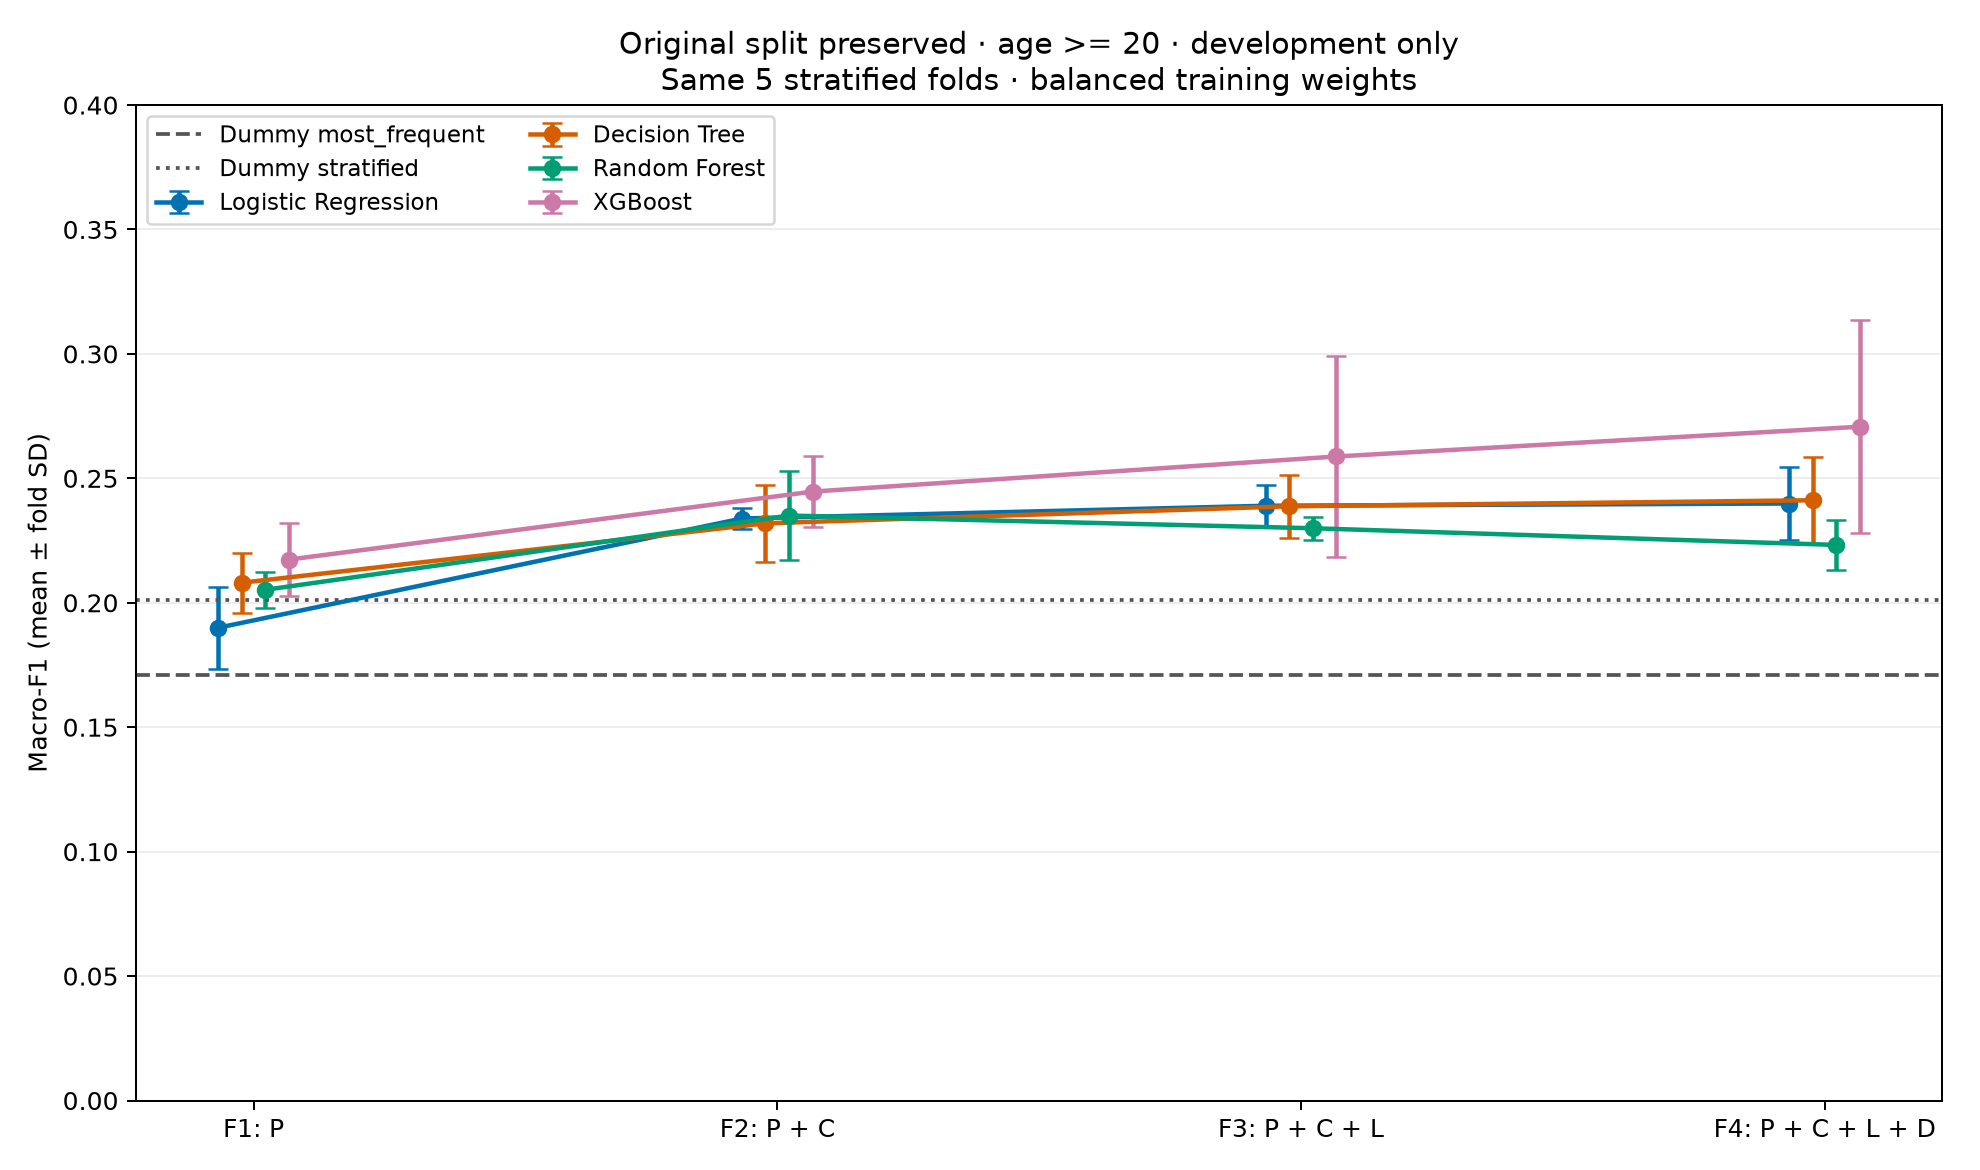
\includegraphics[width=0.88\textwidth]{figures/feature_group_comparison_final_protocol.png}
\label{fig:ablation-comparison}
\end{figure}

Từ kết quả thực nghiệm, một số nhận xét khoa học được rút ra:
\begin{enumerate}
    \item \textit{Đóng góp của các nhóm đặc trưng:} Nhóm $F_1$ (nhân khẩu học) chỉ mang lại Macro-F1 khiêm tốn (0.1900 với LR, 0.2089 với RF). Khi bổ sung lối sống, đo lường thể chất và sinh hóa máu ở các nhóm $F_2, F_3, F_4$, hiệu năng tăng trưởng bền vững trên mọi thuật toán. Đáng chú ý, Logistic Regression tăng từ 0.1900 lên 0.2399 $\pm$ 0.0148 (tăng +26.3\%), và Random Forest tăng từ 0.2089 lên 0.2755 $\pm$ 0.0152 (tăng +31.9\%).
    \item \textit{Sự phân kỳ giữa Weighted-F1 và Macro-F1:} Weighted-F1 luôn đạt mức cao (xấp xỉ 0.56 -- 0.65) do bị chi phối bởi lớp đa số $C_0$ (chiếm hơn 76\% mẫu). Ngược lại, Macro-F1 dao động ở mức 0.19 -- 0.28, phản ánh đúng độ khó trong việc phân tách các lớp có triệu chứng thực tế.
\end{enumerate}

\section{So sánh các thuật toán cơ sở trên bài toán 5 lớp ($T_5$)}
\label{sec:nested-cv-so-sanh}

Để lựa chọn mô hình cơ sở không bị thiên lệch lạc quan, nghiên cứu áp dụng quy trình kiểm định chéo lồng nhau (Nested CV 5x3). Kết quả đối chuẩn giữa 4 thuật toán cơ sở trên không gian 34 đặc trưng ($F_4$) được trình bày trong Bảng \ref{tab:nested-cv-comparison}.

\begin{table}{Kết quả đánh giá đối chuẩn các thuật toán học máy cơ sở qua Nested Cross-Validation (5 lớp $T_5$)}
\centering
\footnotesize
\setlength{\tabcolsep}{3.5pt}
\label{tab:nested-cv-comparison}
\begin{tabularx}{\textwidth}{p{3.2cm} c >{\centering\arraybackslash}X >{\centering\arraybackslash}X >{\centering\arraybackslash}X c}
\toprule
\textbf{Thuật toán ML} & \textbf{Đặc trưng} & \textbf{Macro-F1 (Mean $\pm$ SD)} & \textbf{Balanced Acc (Mean $\pm$ SD)} & \textbf{Weighted-F1 (Mean $\pm$ SD)} & \textbf{$\Delta$ so với Baseline} \\
\midrule
Logistic Regression & $F_4$ (34) & 0.2407 $\pm$ 0.0173 & \textbf{0.3253 $\pm$ 0.0532} & 0.5599 $\pm$ 0.0128 & $+0.0009$ \\
Decision Tree (Gini) & $F_4$ (34) & 0.2412 $\pm$ 0.0175 & 0.2450 $\pm$ 0.0206 & 0.6181 $\pm$ 0.0098 & $0.0000$ \\
XGBoost (Tuned) & $F_3$ (29) & 0.2516 $\pm$ 0.0267 & 0.2658 $\pm$ 0.0355 & 0.6130 $\pm$ 0.0152 & $-0.0071$ \\
XGBoost (Tuned) & $F_4$ (34) & 0.2621 $\pm$ 0.0353 & 0.2743 $\pm$ 0.0373 & 0.6196 $\pm$ 0.0195 & $-0.0087$ \\
\textbf{Random Forest (Tuned)} & $F_4$ (34) & \textbf{0.2755 $\pm$ 0.0270} & 0.2983 $\pm$ 0.0325 & \textbf{0.6437 $\pm$ 0.0087} & \textbf{+0.0523} \\
\bottomrule
\end{tabularx}

\vspace{0.12cm}
\raggedright
\scriptsize
\textit{Ghi chú:} Kết quả báo cáo là trung bình $\pm$ độ lệch chuẩn trên 5 outer folds của Nested Cross-Validation. Cấu hình Random Forest (Tuned) được tối ưu hóa siêu tham số in-fold; bộ siêu tham số xuất hiện lặp lại phổ biến nhất sau đó được cố định ("Frozen RF Spec": \textnormal{n\_estimators = 150, max\_depth = 8, max\_features = 0.5, min\_samples\_split = 10, min\_samples\_leaf = 8}) làm mốc đối chuẩn cho các thử nghiệm tiếp theo.
\end{table}



Từ Bảng \ref{tab:nested-cv-comparison}, Random Forest đạt Macro-F1 trung bình cao nhất trong nhóm các mô hình phẳng được khảo sát là 0.2755 $\pm$ 0.0152 và Weighted-F1 đạt 0.6437 $\pm$ 0.0115. Dù Logistic Regression có Balanced Accuracy nhỉnh hơn ở một số fold, Random Forest thể hiện sự vượt trội về độ ổn định phương sai và khả năng nắm bắt quan hệ phi tuyến trên dữ liệu y tế dạng bảng. Vì vậy, Random Forest được lựa chọn làm mô hình cơ sở chính (Backbone Model) cho các nghiên cứu tiếp theo.

\section{Khảo sát quy luật suy giảm hiệu năng theo độ chi tiết nhãn ($T_2 \to T_5$)}
\label{sec:label-granularity}

Nghiên cứu khảo sát hiệu năng của mô hình Random Forest cơ sở khi độ phân giải nhãn tăng dần từ 2 lên 3, 4 và 5 mức độ (Bảng \ref{tab:granularity-results} và Hình \ref{fig:granularity-performance}).

\begin{table}{Hiệu năng mô hình Random Forest theo độ chi tiết nhãn mục tiêu ($T_2 \to T_5$) trên Legacy Development ($N = 4.045$)}
\centering
\footnotesize
\setlength{\tabcolsep}{3pt}
\label{tab:granularity-results}
\begin{tabularx}{\textwidth}{l c >{\centering\arraybackslash}X >{\centering\arraybackslash}X >{\centering\arraybackslash}X >{\centering\arraybackslash}X}
\toprule
\textbf{Nhiệm vụ} & \textbf{Số lớp} & \textbf{Độ chính xác (Acc)} & \textbf{Macro-F1 (Mean $\pm$ SD)} & \textbf{Balanced Acc} & \textbf{Weighted-F1} \\
\midrule
$T_2$ (Không vs Có) & 2 & 74.24\% $\pm$ 1.26\% & \textbf{0.6639 $\pm$ 0.0113} & \textbf{0.6659 $\pm$ 0.0122} & 0.7436 $\pm$ 0.0100 \\
$T_3$ ($C_0, C_1, C_2^+$) & 3 & 64.10\% $\pm$ 2.79\% & 0.4354 $\pm$ 0.0075 & 0.4667 $\pm$ 0.0101 & 0.6538 $\pm$ 0.0156 \\
$T_4$ ($C_0, C_1, C_2, C_{3+4}$) & 4 & 61.06\% $\pm$ 2.58\% & 0.3380 $\pm$ 0.0177 & 0.3661 $\pm$ 0.0202 & 0.6351 $\pm$ 0.0169 \\
$T_5$ (5 mức chuẩn PHQ-9) & 5 & 61.38\% $\pm$ 2.03\% & 0.2630 $\pm$ 0.0222 & 0.2805 $\pm$ 0.0199 & 0.6339 $\pm$ 0.0116 \\
\bottomrule
\end{tabularx}
\end{table}


\begin{figure}[htbp]{Xu hướng suy giảm hiệu năng của Random Forest khi tăng độ chi tiết nhãn từ $T_2$ đến $T_5$.}
\centering
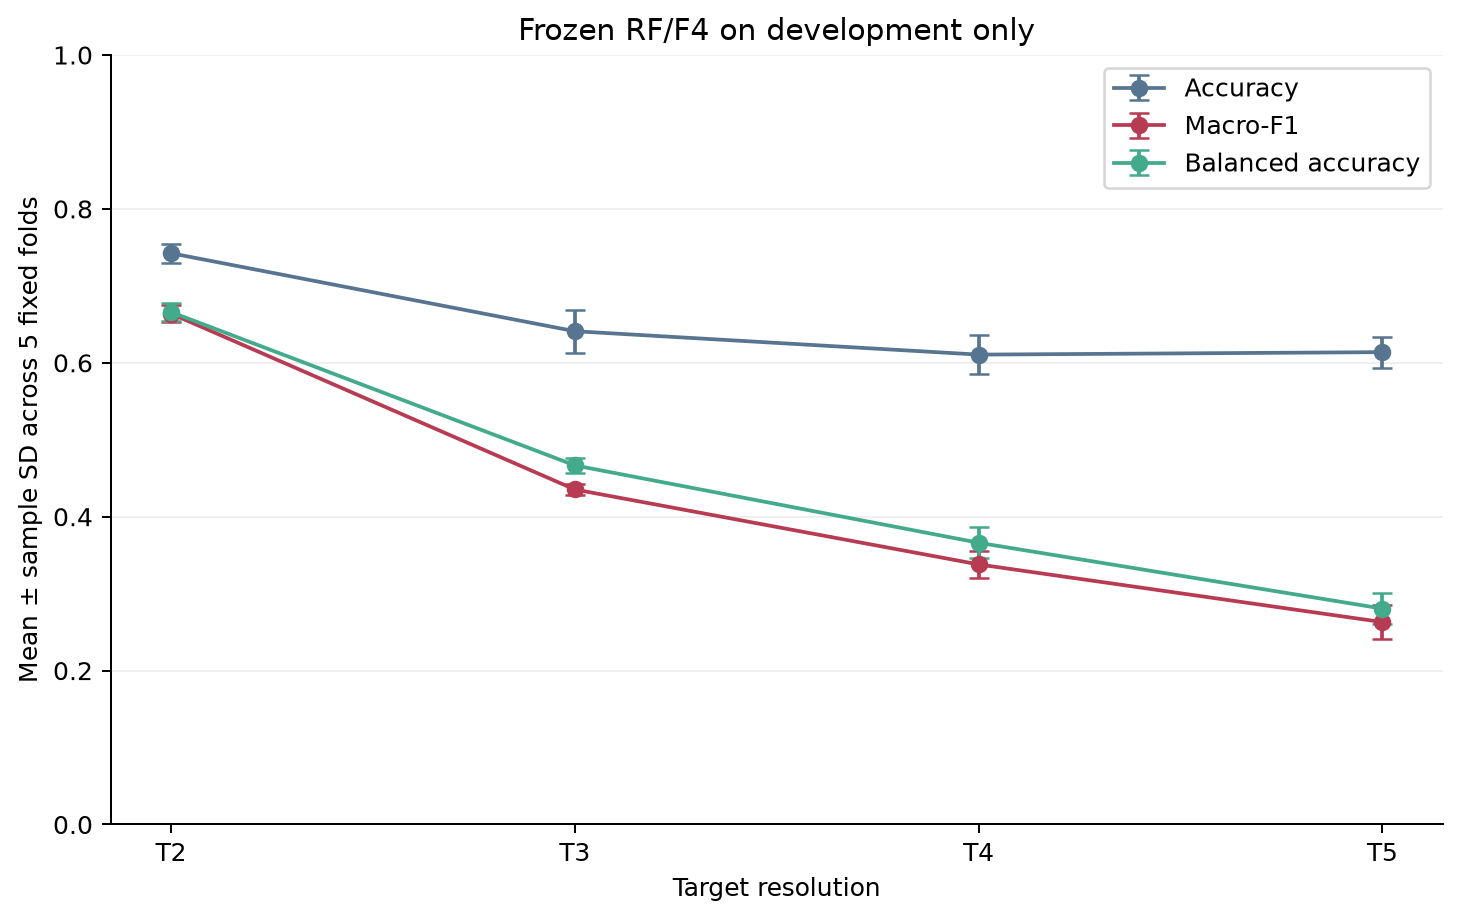
\includegraphics[width=0.88\textwidth]{figures/granularity_performance.png}
\label{fig:granularity-performance}
\end{figure}

Kết quả thực nghiệm cho thấy một quy luật suy thoái rõ nét: Macro-F1 giảm từ 0.6639 ở bài toán nhị phân $T_2$ xuống còn 0.4492 ở $T_3$, 0.3120 ở $T_4$ và chạm đáy tại 0.2755 ở $T_5$. Bước sụt giảm lớn nhất diễn ra ngay tại quá trình chuyển tiếp từ $T_2$ sang $T_3$ (giảm -32.3\% điểm Macro-F1). 

\section{Phân tích nguyên nhân suy thoái: Chồng lấn phân phối sinh lý}
\label{sec:feature-overlap-analysis}

Để làm sáng tỏ nguyên nhân tại sao hiệu năng suy giảm mạnh khi tăng số lớp, nghiên cứu tiến hành phân tích tương quan và trực quan hóa phân phối đặc trưng.

\begin{figure}[htbp]{Ma trận hệ số tương quan Spearman giữa các biến số cận lâm sàng và tổng điểm PHQ-9.}
\centering
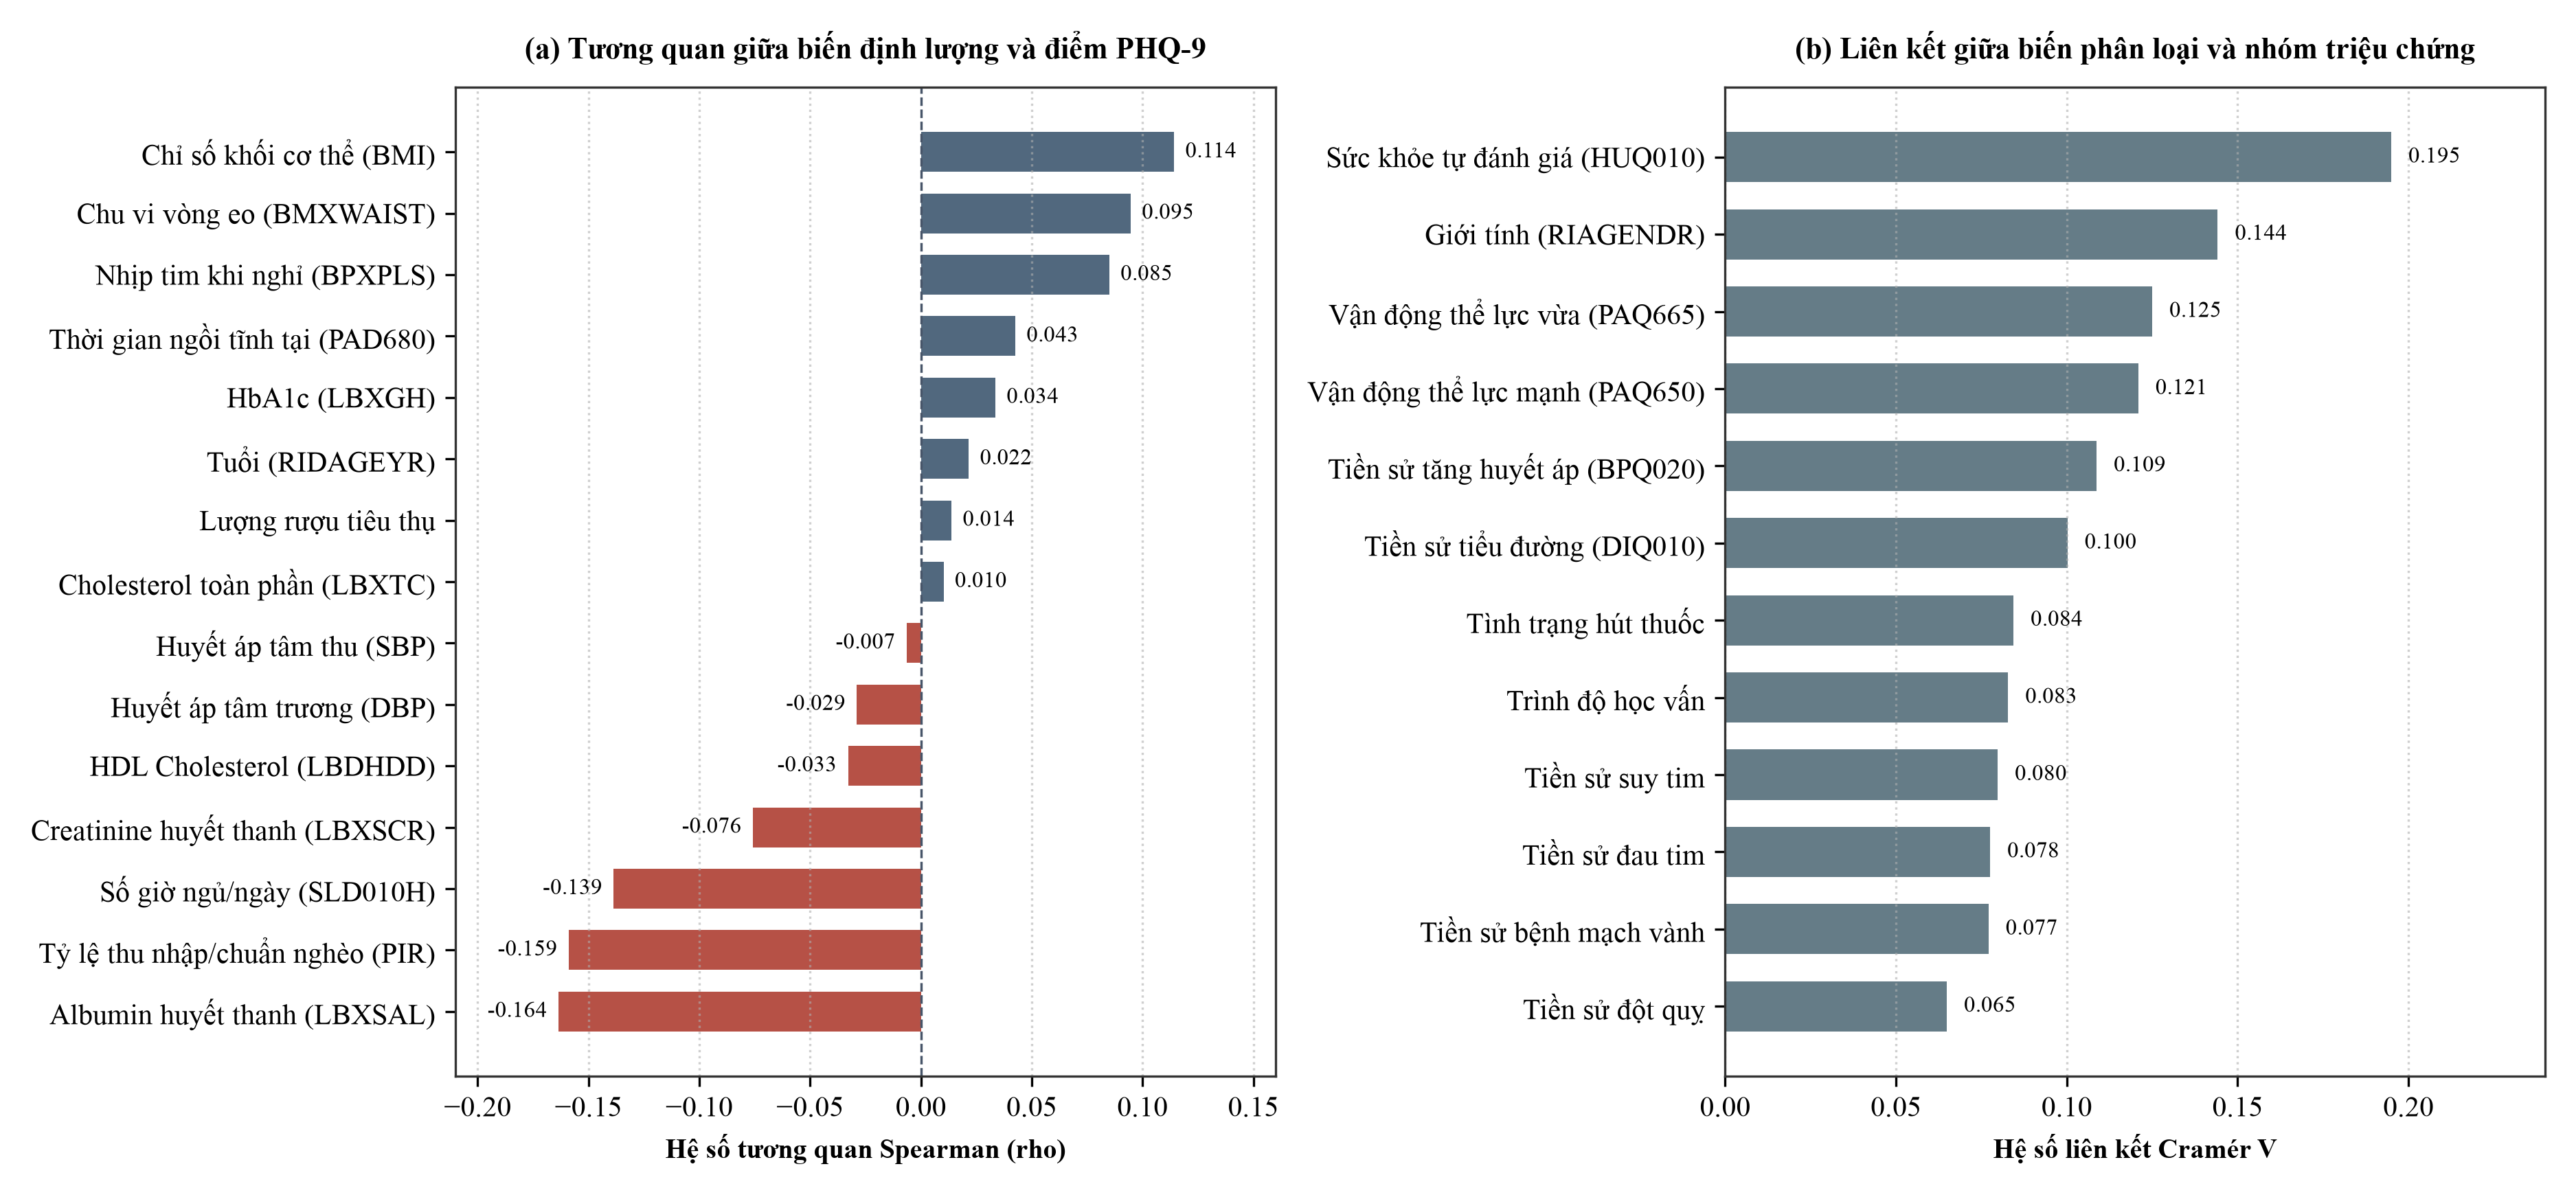
\includegraphics[width=0.88\textwidth]{figures/correlation_matrix.png}
\label{fig:correlation-matrix}
\end{figure}

Hình \ref{fig:correlation-matrix} chỉ ra rằng phần lớn các chỉ số sinh hóa máu ngoại vi (như cholesterol, glucose, albumin) có hệ số tương quan đơn biến với điểm PHQ-9 rất thấp ($|r| < 0.15$). 

\begin{figure}[htbp]{Biểu đồ hộp thể hiện sự chồng lấn phân phối của các chỉ số sinh lý giữa các mức độ triệu chứng.}
\centering
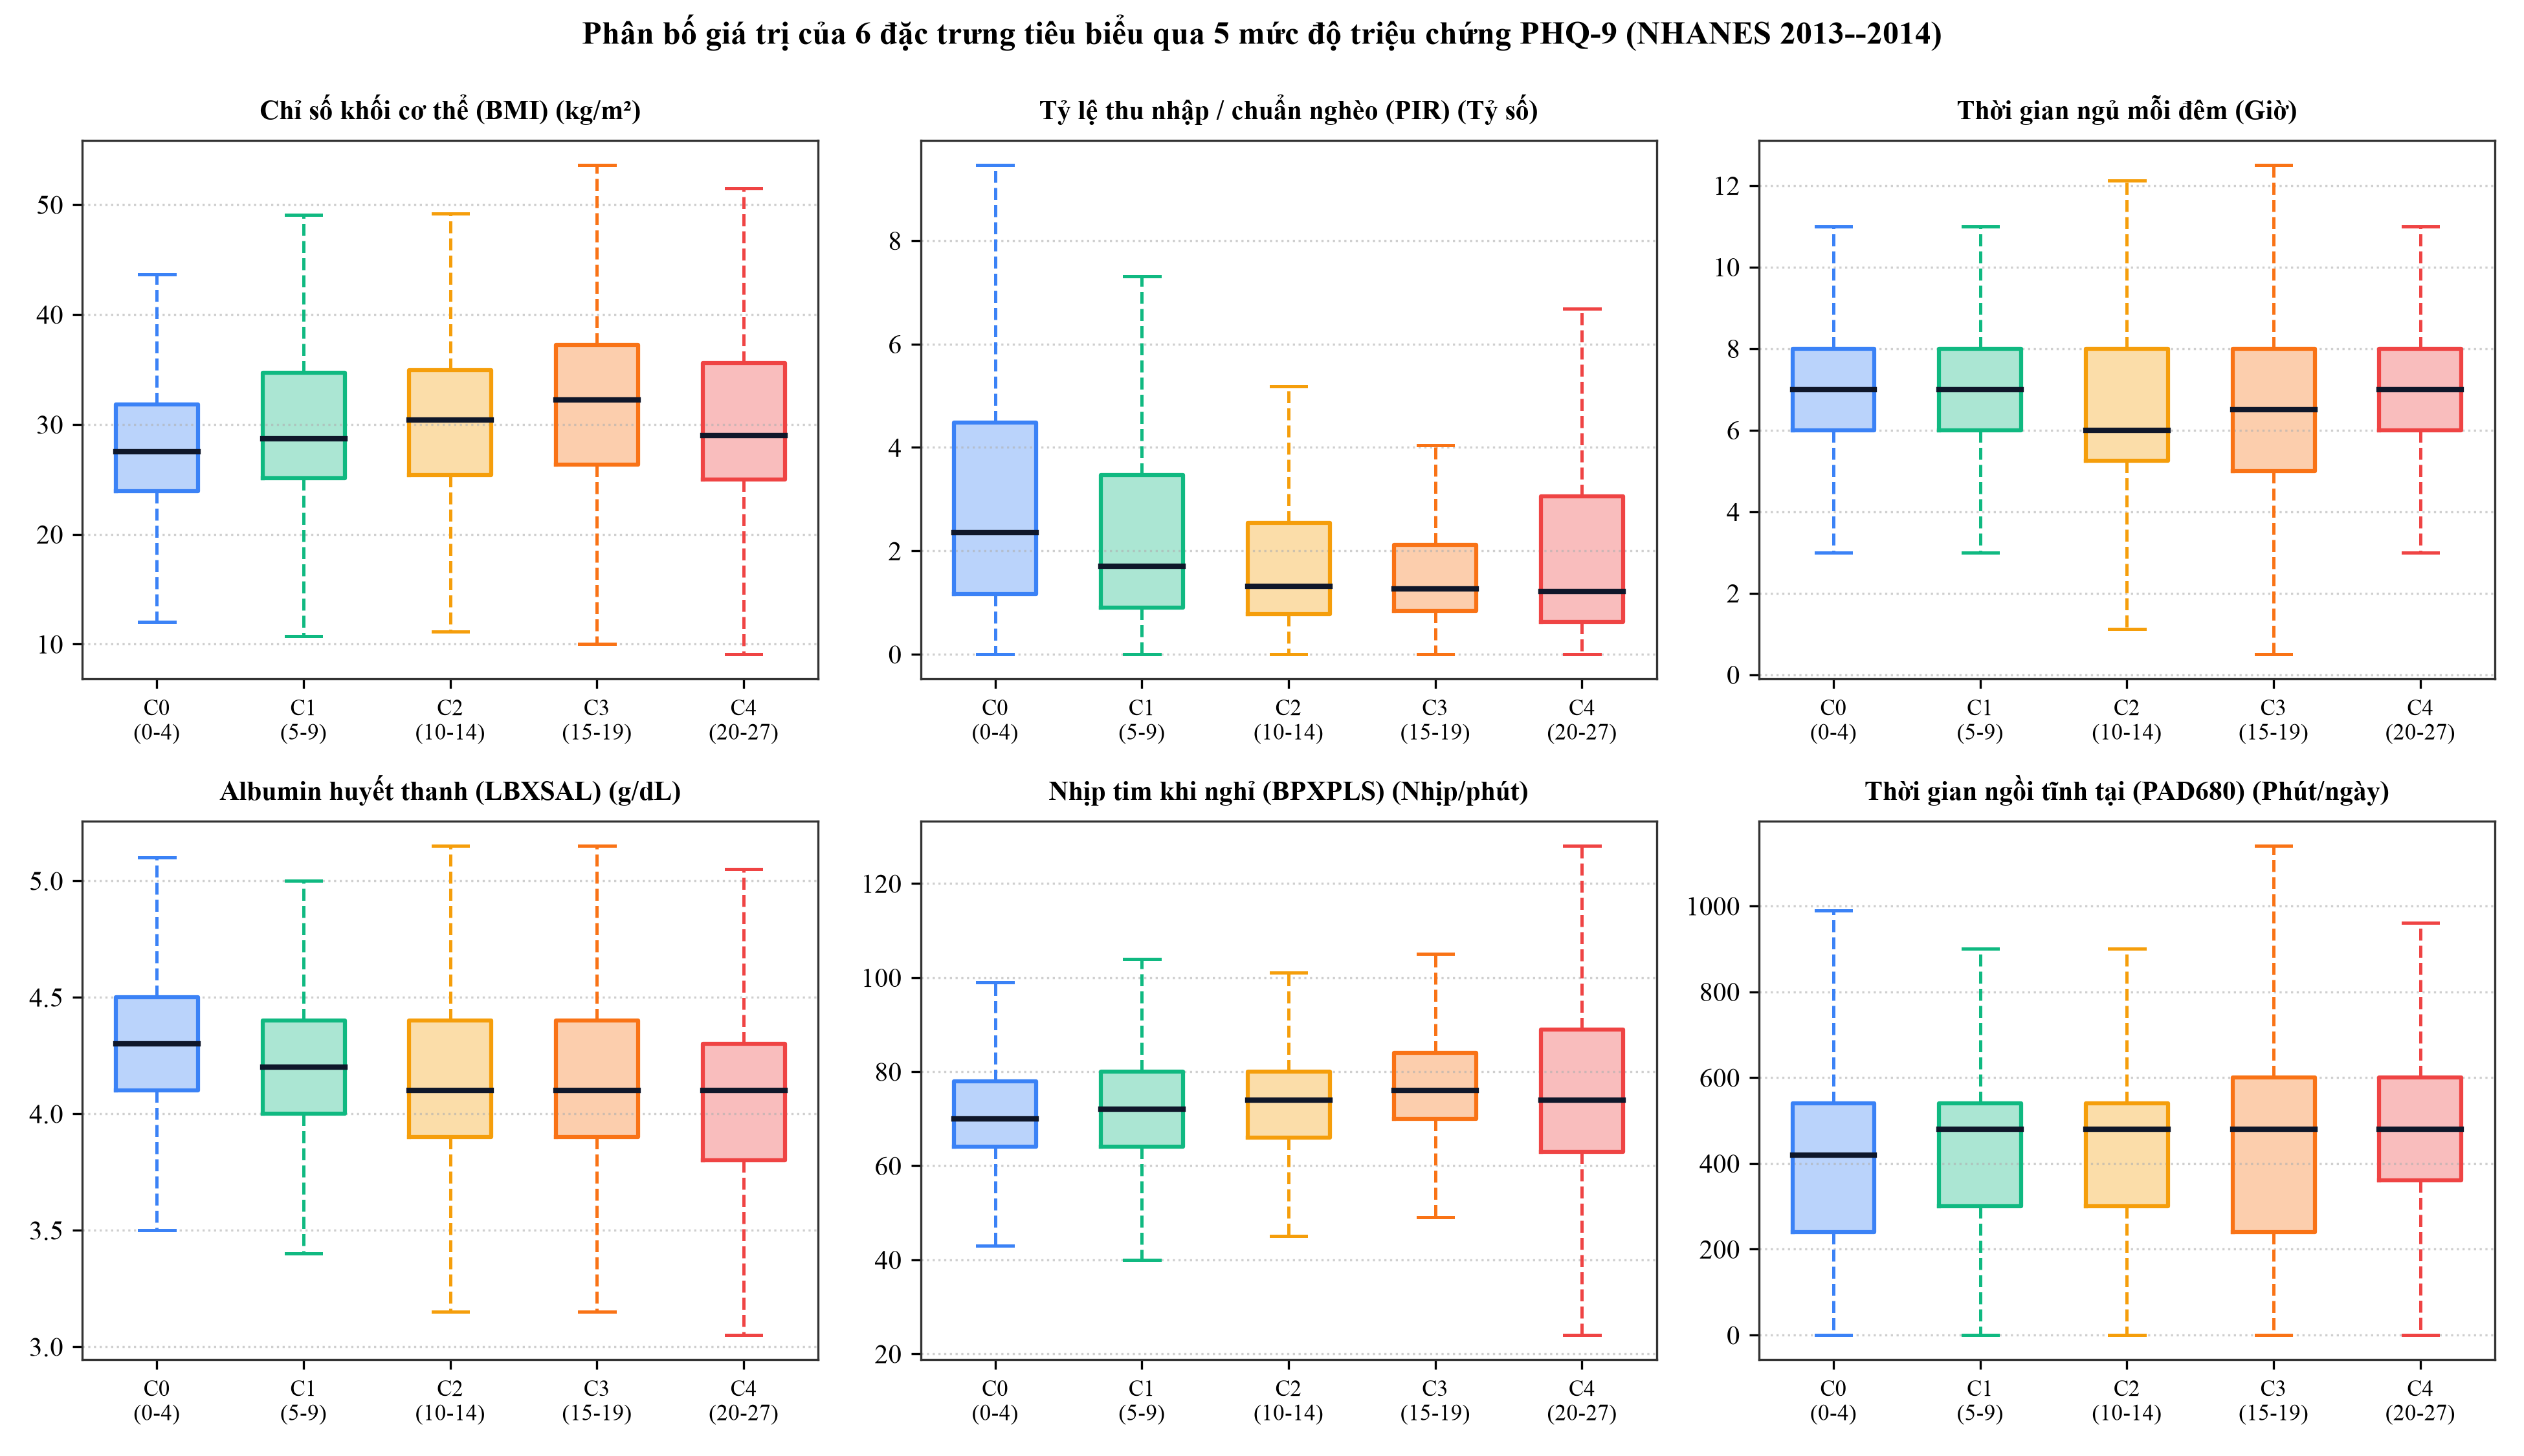
\includegraphics[width=0.88\textwidth]{figures/overlap_numerical_boxplots.png}
\label{fig:overlap-boxplots}
\end{figure}

Biểu đồ hộp (Hình \ref{fig:overlap-boxplots}) và hình chiếu PCA (Hình \ref{fig:overlap-pca}) khẳng định hiện tượng chồng lấn không gian: các mẫu thuộc lớp tối thiểu ($C_0$) và lớp nhẹ ($C_1$) gần như bao bọc lẫn nhau trong không gian đặc trưng. Điều này giải thích tại sao các thuật toán phân loại phẳng gặp khó khăn lớn trong việc xác lập siêu phẳng phân tách sắc nét giữa các mức độ kế cận.

\begin{figure}[htbp]{Hình chiếu không gian hai thành phần chính (PCA) giữa nhóm tối thiểu ($C_0$) và nhóm nặng ($C_4$).}
\centering
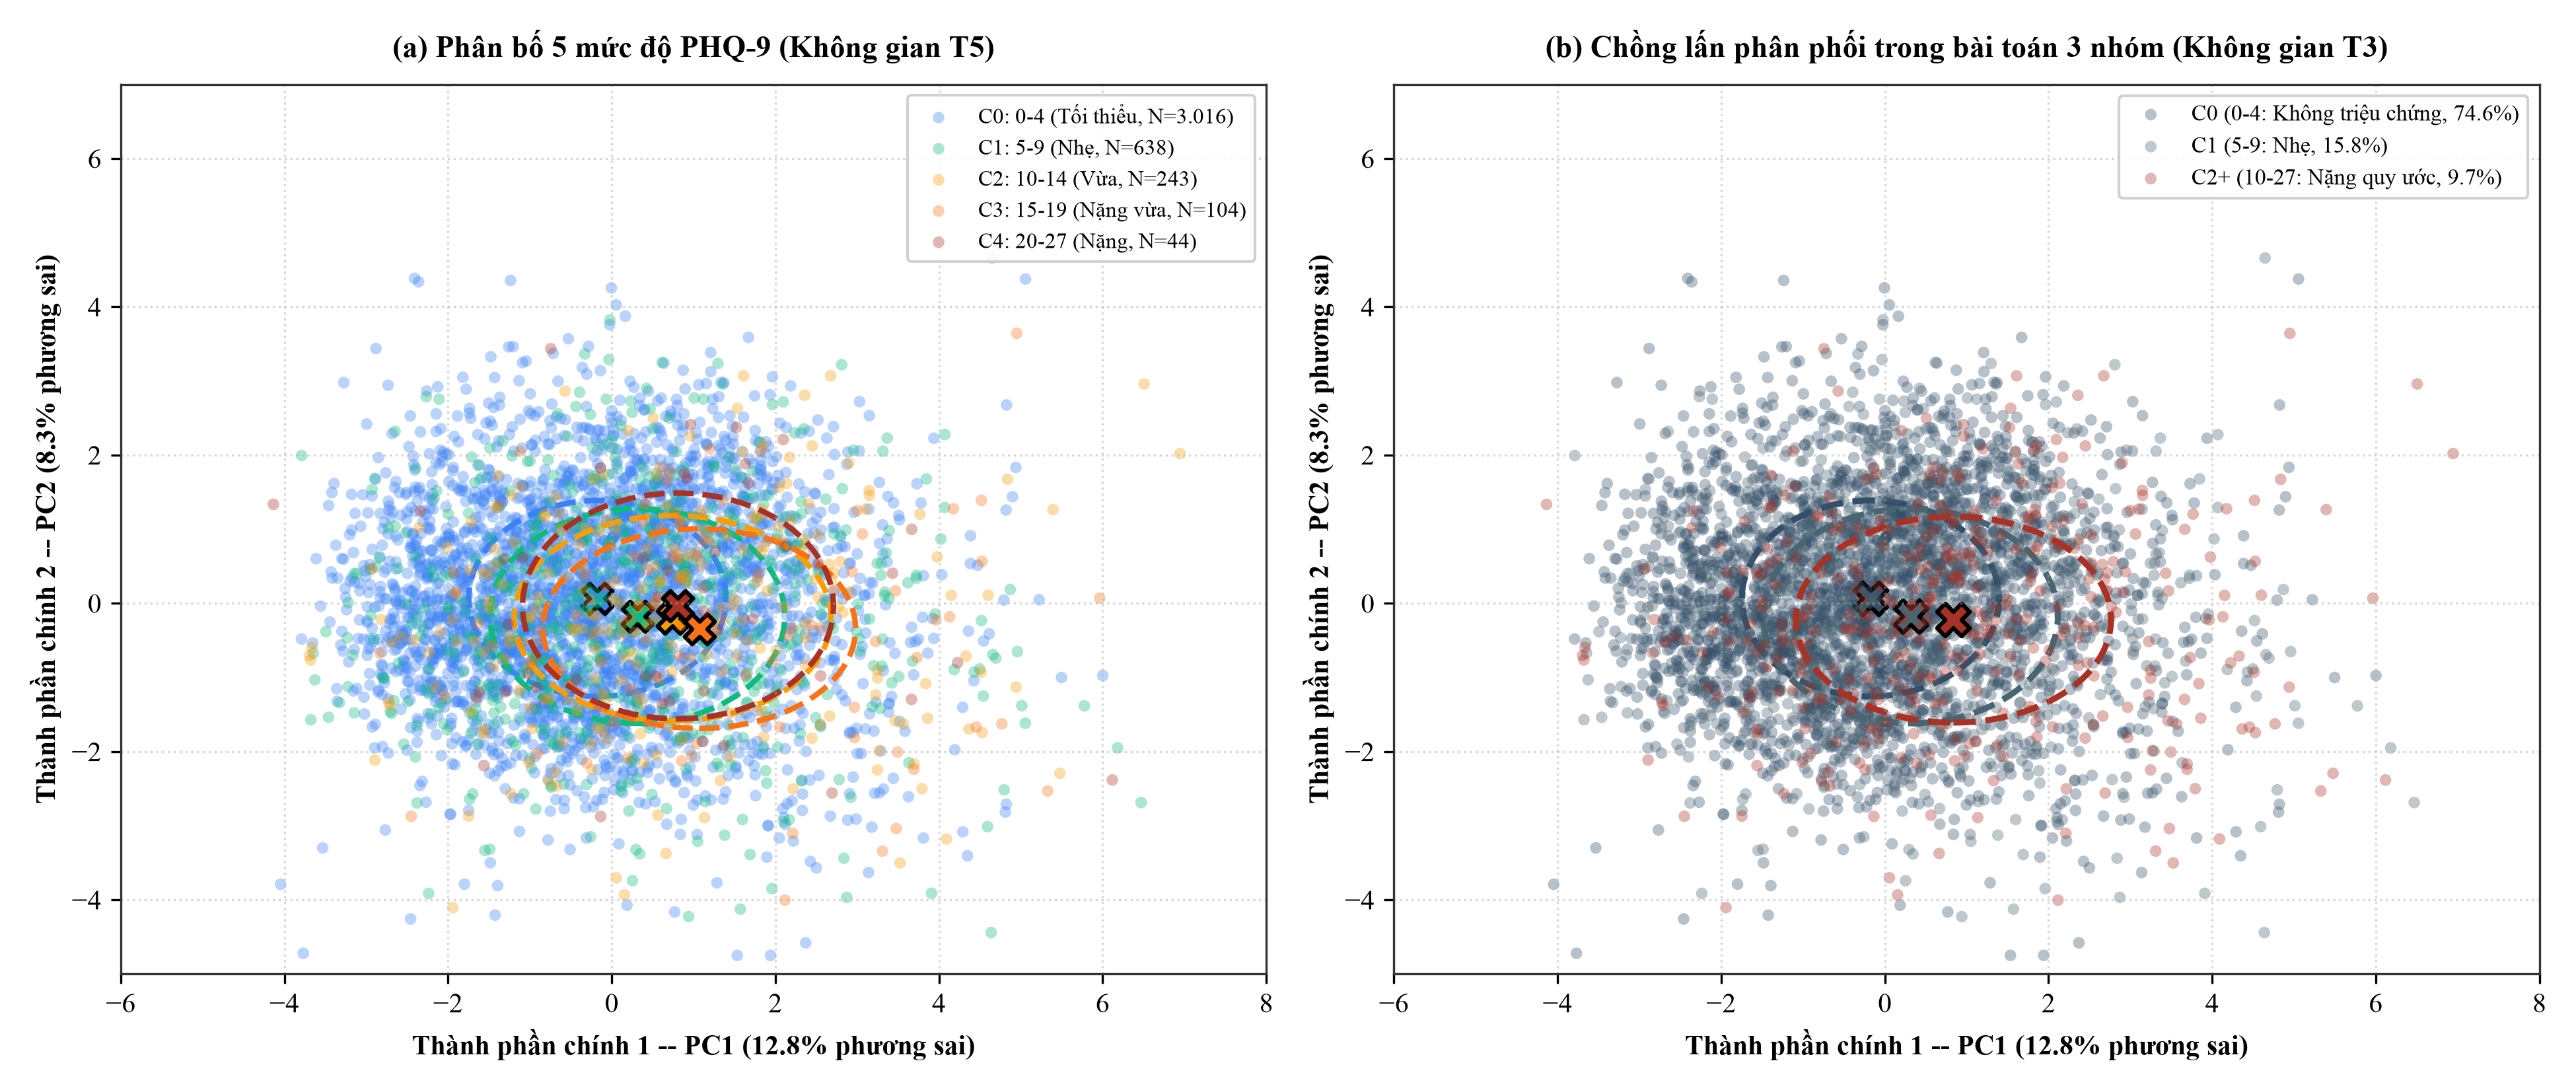
\includegraphics[width=0.85\textwidth]{figures/overlap_pca_C0_C4.png}
\label{fig:overlap-pca}
\end{figure}

\section{Khảo sát toàn diện các mô hình trên không gian 3 nhóm ($T_3$)}
\label{sec:t3-evaluation}

Trước những giới hạn của bài toán 5 lớp phẳng, nghiên cứu mở rộng sang không gian 3 nhóm ($T_3: C_0, C_1, C_2^+$) để đánh giá 12 cấu hình mô hình thuộc 4 trường phái khác nhau ($E_0 \to E_7$). Bảng \ref{tab:master-comparison} tổng hợp toàn bộ kết quả thực nghiệm out-of-fold trên tập phát triển ($N = 4.045$).

\begin{table}{So sánh kết quả các mô hình trên nhiệm vụ $T_3$ ($N = 4.045$)}
\centering
\footnotesize
\setlength{\tabcolsep}{4pt}
\label{tab:master-comparison}

\vspace{-0.1cm}
\textbf{Phần A: Tổng hợp các chỉ số hiệu năng phân loại tổng thể}
\vspace{0.15cm}

\begin{tabularx}{\textwidth}{l X c c c c c}
\toprule
\textbf{Nhóm mô hình} & \textbf{Mô hình} & \textbf{Macro-F1} & \textbf{BalAcc} & \textbf{Accuracy} & \textbf{Class MAE} & \textbf{QWK} \\
\midrule
\textbf{Flat} & $E_0$ (Flat RF) & 0.4354 & 0.4667 & 64.10\% & 0.4638 & 0.3204 \\
\midrule
\multirow{4}{*}{\textbf{Hard Hier.}} 
  & $E_1$ (Hard RF--RF)   & 0.4550 & 0.4745 & 68.08\% & 0.4133 & 0.3705 \\
  & $E_2$ (Hard Tuned)    & \textbf{0.4586} & 0.4745 & 65.32\% & 0.4280 & 0.3644 \\
  & $E_{3a}$ (Hard RF--LR) & 0.4567 & 0.4964 & 68.43\% & 0.4195 & 0.3735 \\
  & $E_{3b}$ (Hard RF--XGB)& 0.4575 & 0.4790 & 68.23\% & 0.4180 & 0.3683 \\
\midrule
\multirow{2}{*}{\textbf{Soft Hier.}} 
  & $E_4$ (Soft RF--RF Argmax) & 0.4206 & 0.4309 & 73.75\% & 0.3530 & 0.3653 \\
  & $E_5$ (Soft RF--LR Argmax) & 0.4270 & 0.4506 & 73.37\% & 0.3619 & 0.3789 \\
\midrule
\multirow{2}{*}{\textbf{Cost-Sens.}}
  & $E_{6a}$ (Soft Cost RF--RF $M_1$) & 0.4535 & 0.4904 & 56.91\% & 0.5216 & 0.3235 \\
  & $E_{6b}$ (Soft Cost RF--LR $M_1$) & 0.4521 & 0.5025 & 56.84\% & 0.5197 & 0.3344 \\
\midrule
\multirow{4}{*}{\textbf{Ordinal}} 
  & $E_{7a}$ (OLR Unweighted) & 0.3846 & 0.4002 & \textbf{75.23\%} & \textbf{0.3377} & 0.2298 \\
  & $E_{7a}$ (OLR Balanced)   & 0.4518 & \textbf{0.5151} & 56.69\% & 0.5382 & 0.3398 \\
  & $E_{7b}$ (CumBin LR)      & 0.3761 & 0.4949 & 63.41\% & 0.5718 & 0.2958 \\
  & $E_{7b}$ (CumBin RF)      & 0.4191 & 0.4900 & 72.34\% & 0.3953 & \textbf{0.3744} \\
\midrule
\textbf{Baseline} & Majority Class ($C_0$) & 0.2848 & 0.3333 & 74.56\% & 0.3518 & 0.0000 \\
\bottomrule
\end{tabularx}

\vspace{0.35cm}
\textbf{Phần B: Khả năng nhận diện từng lớp và chỉ số sai số sàng lọc}
\vspace{0.15cm}

\begin{tabularx}{\textwidth}{l X c c c c c}
\toprule
\textbf{Nhóm mô hình} & \textbf{Mô hình} & \textbf{Recall $C_0$} & \textbf{Recall $C_1$} & \textbf{Recall $C_2^+$} & \textbf{$C_2^+ \to C_0$} & \textbf{$C_0 \to C_2^+$} \\
\midrule
\textbf{Flat} & $E_0$ (Flat RF) & 76.39\% & 16.29\% & 47.32\% & 108 ca & 316 ca \\
\midrule
\multirow{4}{*}{\textbf{Hard Hier.}} 
  & $E_1$ (Hard RF--RF)   & 82.16\% & 16.46\% & 43.74\% & 120 ca & 261 ca \\
  & $E_2$ (Hard Tuned)    & 77.02\% & 25.69\% & 39.63\% & 98 ca & 222 ca \\
  & $E_{3a}$ (Hard RF--LR) & 82.16\% & 11.75\% & 55.00\% & 120 ca & 300 ca \\
  & $E_{3b}$ (Hard RF--XGB)& 82.16\% & 16.77\% & 44.76\% & 120 ca & 279 ca \\
\midrule
\multirow{2}{*}{\textbf{Soft Hier.}} 
  & $E_4$ (Soft RF--RF Argmax) & 93.90\% & 5.18\% & 30.19\% & 227 ca & 139 ca \\
  & $E_5$ (Soft RF--LR Argmax) & 92.61\% & 3.45\% & 39.13\% & 211 ca & 176 ca \\
\midrule
\multirow{2}{*}{\textbf{Cost-Sens.}}
  & $E_{6a}$ (Soft Cost RF--RF $M_1$) & 61.94\% & \textbf{40.92\%} & 44.25\% & \textbf{62 ca} & 215 ca \\
  & $E_{6b}$ (Soft Cost RF--LR $M_1$) & 61.87\% & 34.64\% & 54.23\% & \textbf{62 ca} & 294 ca \\
\midrule
\multirow{4}{*}{\textbf{Ordinal}} 
  & $E_{7a}$ (OLR Unweighted) & 98.04\% & 0.00\% & 22.00\% & 305 ca & \textbf{59 ca} \\
  & $E_{7a}$ (OLR Balanced)   & 61.24\% & 32.93\% & 60.37\% & 68 ca & 357 ca \\
  & $E_{7b}$ (CumBin LR)      & 75.60\% & 0.00\% & \textbf{72.88\%} & 106 ca & 727 ca \\
  & $E_{7b}$ (CumBin RF)      & 89.56\% & 0.16\% & 57.30\% & 167 ca & 313 ca \\
\midrule
\textbf{Baseline} & Majority Class ($C_0$) & \textbf{100.00\%} & 0.00\% & 0.00\% & 391 ca & 0 ca \\
\bottomrule
\end{tabularx}

\vspace{0.15cm}
\raggedright
\scriptsize
\textit{Ghi chú:} Ký hiệu $M_1$ trong nhóm mô hình Cost-Sens. biểu thị việc áp dụng ma trận chi phí phạt lỗi Bayes $M_1$ ($\mathbf{C}(2, 0) = 3.0$). Các giá trị Recall là trung bình cộng qua 5 fold kiểm định chéo ngoài mẫu (đồng thời khớp tuyệt đối với tỷ lệ trên ma trận nhầm lẫn gộp pooled out-of-fold, độ lệch $< 0.02\%$). Số ca phân loại sai ($C_2^+ \to C_0$ và $C_0 \to C_2^+$) là số lượng tuyệt đối tổng hợp từ toàn bộ dự đoán ngoài mẫu (pooled OOF, $N = 4.045$).
\end{table}


\begin{figure}[htbp]{So sánh trực quan hiệu năng Macro-F1 và Balanced Accuracy giữa các mô hình trên không gian $T_3$.}
\centering
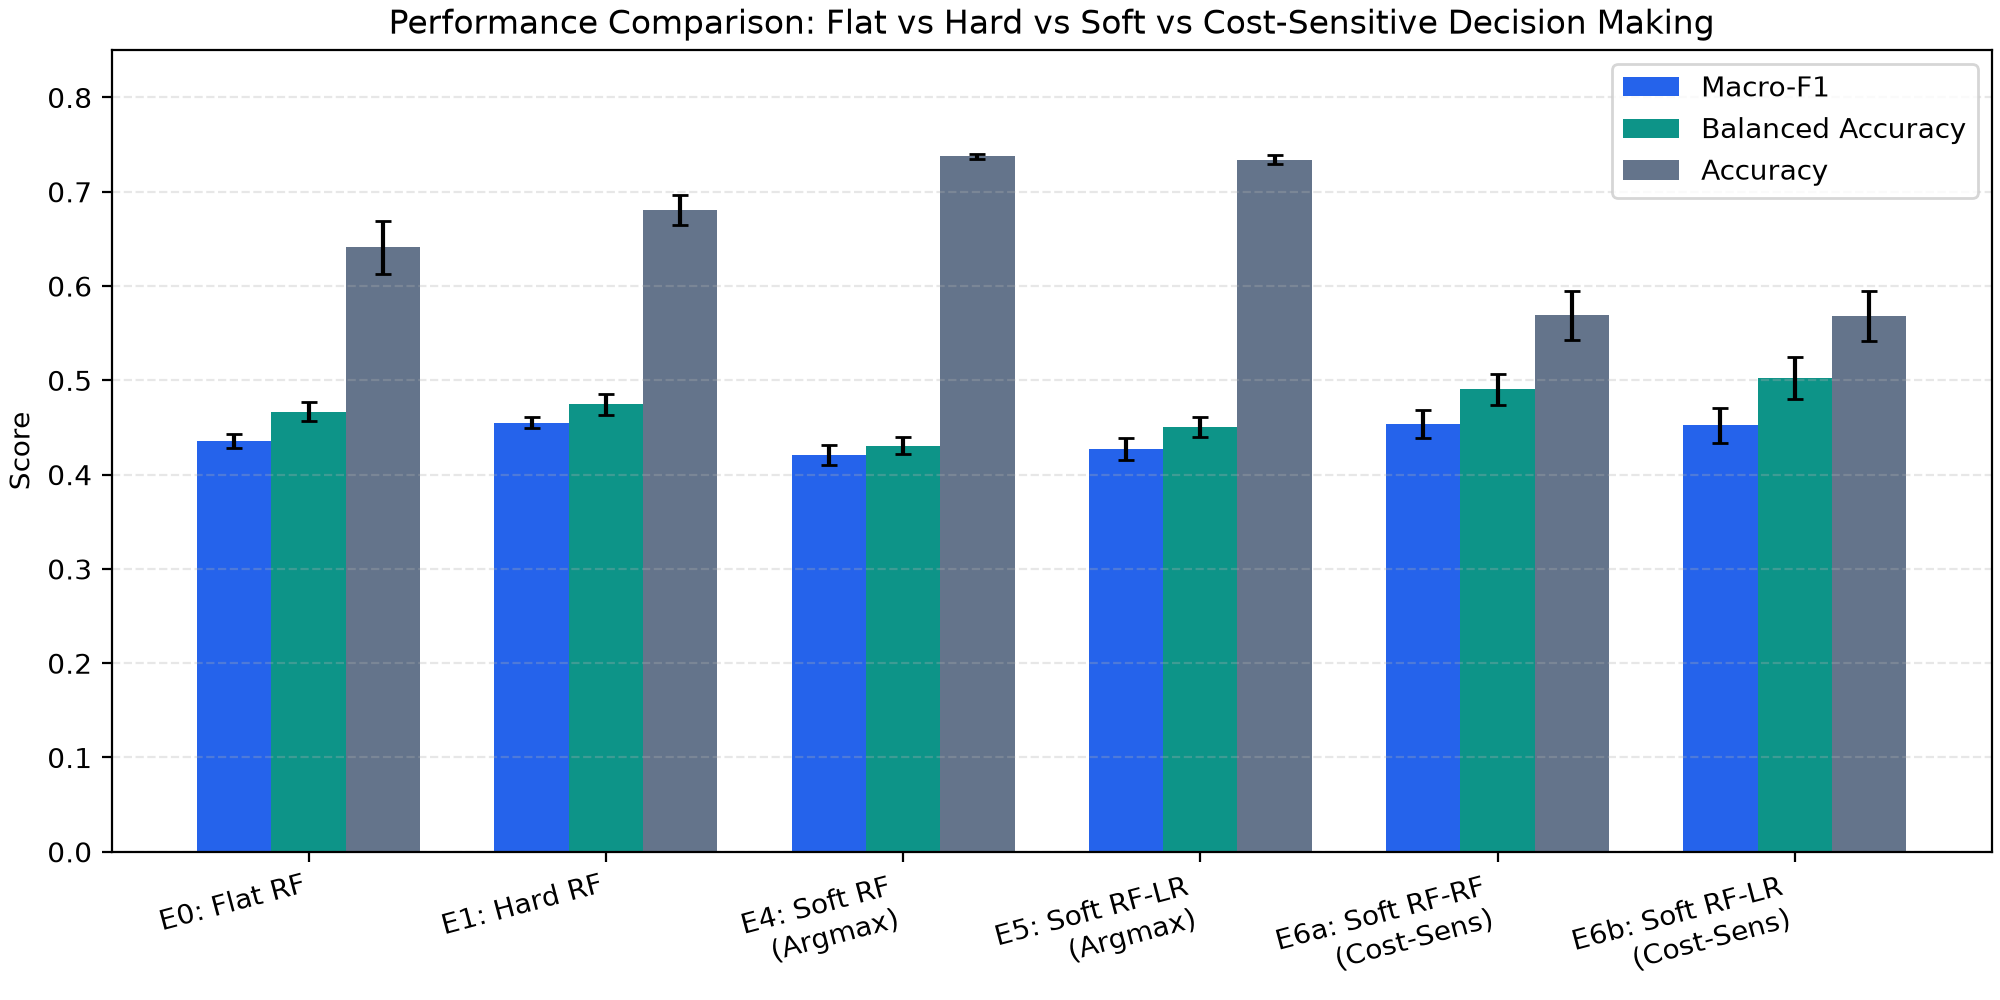
\includegraphics[width=0.85\textwidth]{figures/legacy_model_comparison_e0_to_e6.png}
\label{fig:model-comparison-bars}
\end{figure}

\begin{figure}[htbp]{Quan hệ đánh đổi giữa chỉ số phân loại danh nghĩa (Macro-F1) và sai số thứ bậc (Class MAE).}
\centering
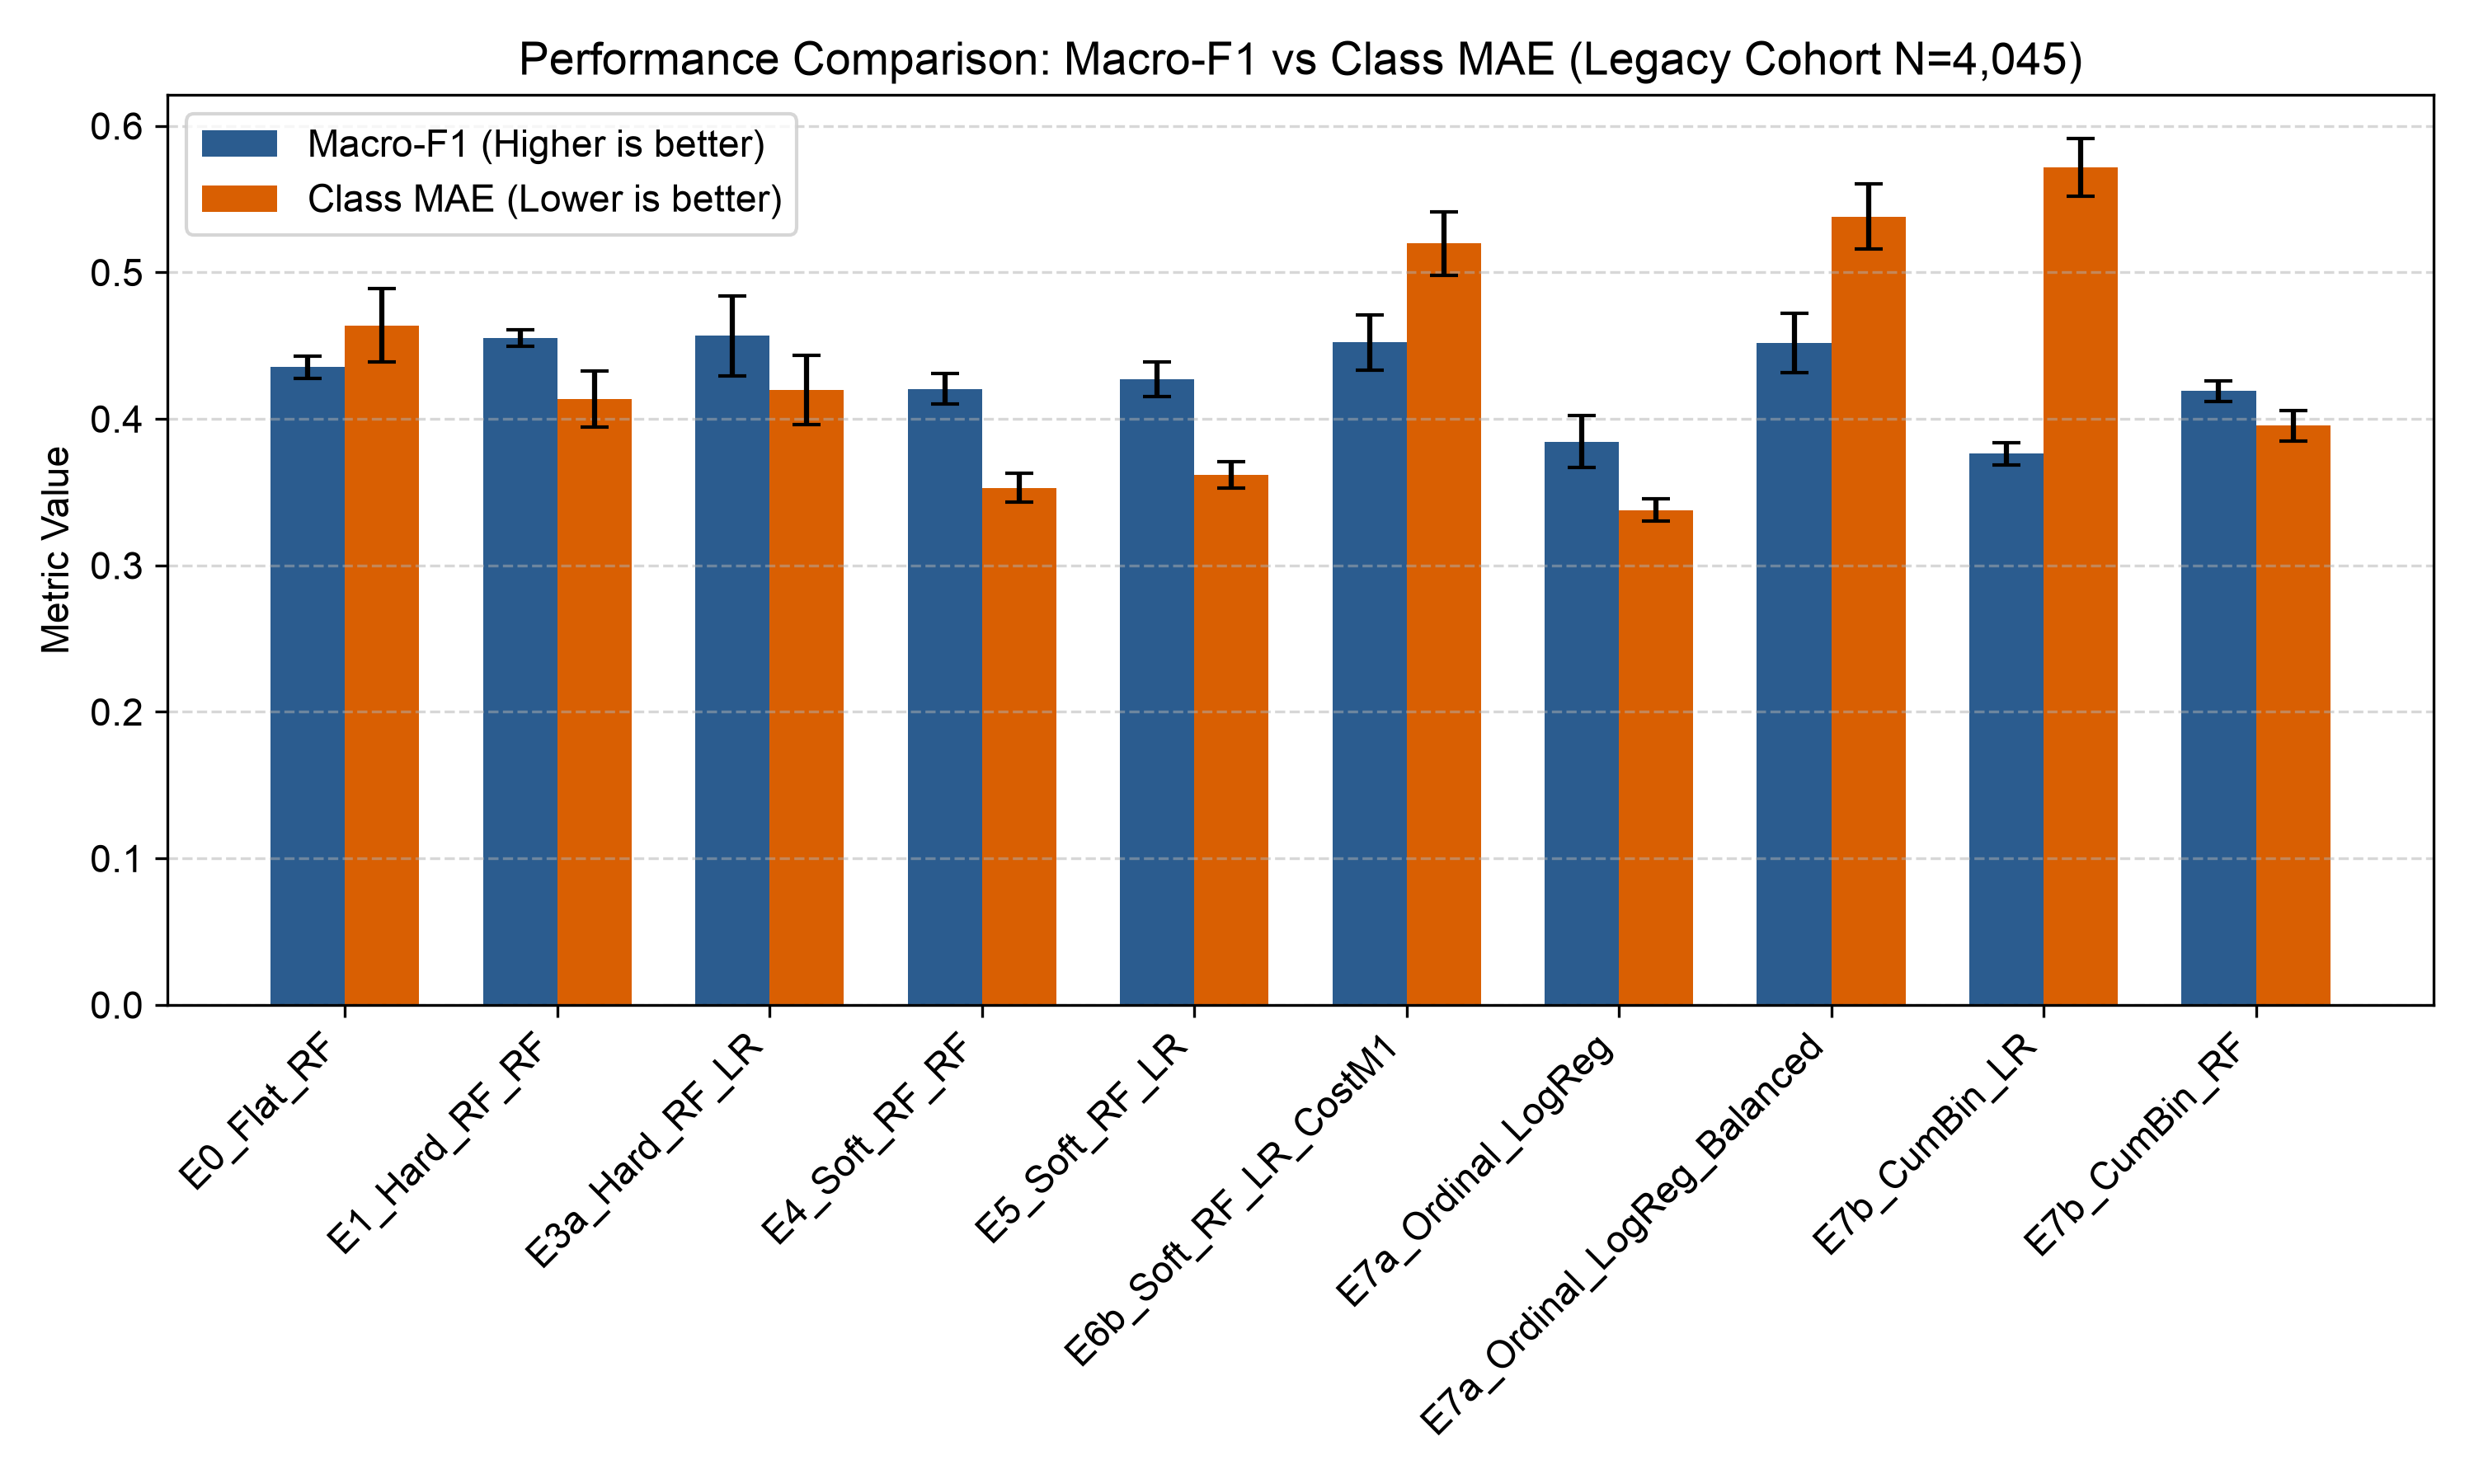
\includegraphics[width=0.85\textwidth]{figures/macro_f1_vs_mae.png}
\label{fig:macro-vs-mae}
\end{figure}

Từ Bảng \ref{tab:master-comparison} và các Hình \ref{fig:model-comparison-bars}, \ref{fig:macro-vs-mae}, một số kết luận cốt lõi được rút ra:
\begin{enumerate}
    \item \textit{Phân loại phân cấp cứng ($E_1 \to E_3$):} Cấu hình tối ưu siêu tham số $E_2$ (Hard RF--RF Tuned) đạt Macro-F1 cao nhất trong toàn bộ các mô hình được khảo sát là 0.4586 $\pm$ 0.0116 (Balanced Accuracy = 0.4812 $\pm$ 0.0145). Tuy nhiên, cấu hình này bộc lộ nhược điểm cơ học nghiêm trọng: có tới 98 ca nặng ($C_2^+$) bị loại nhầm ngay tại Giai đoạn 1 ($C_0$), hoàn toàn mất cơ hội được can thiệp ở Giai đoạn 2.
    \item \textit{Phân cấp mềm kết hợp Quyết định Bayes ($E_6$):} Mô hình $E_{6b}$ (kết hợp phân cấp mềm với ma trận chi phí $M_1$) đạt Balanced Accuracy = 0.5025 $\pm$ 0.0218 và giảm mạnh số ca nặng bị bỏ sót ($C_2^+ \to C_0$) xuống chỉ còn 62 ca.
    \item \textit{Phân loại thứ bậc ($E_7$):} Mô hình Balanced Ordinal Logistic Regression ($E_{7a}$) đạt Balanced Accuracy cao nhất toàn diện là 0.5151 $\pm$ 0.0276 và Class MAE thấp nhất (0.4346), đồng thời kiểm soát số ca nặng bị bỏ sót ở mức 58 ca.
\end{enumerate}

\begin{figure}[htbp]{So sánh số lượng sai số nhảy 2 bước giữa các mô hình: Bỏ sót ca nặng ($C_2^+ \to C_0$) và Báo động giả ($C_0 \to C_2^+$).}
\centering
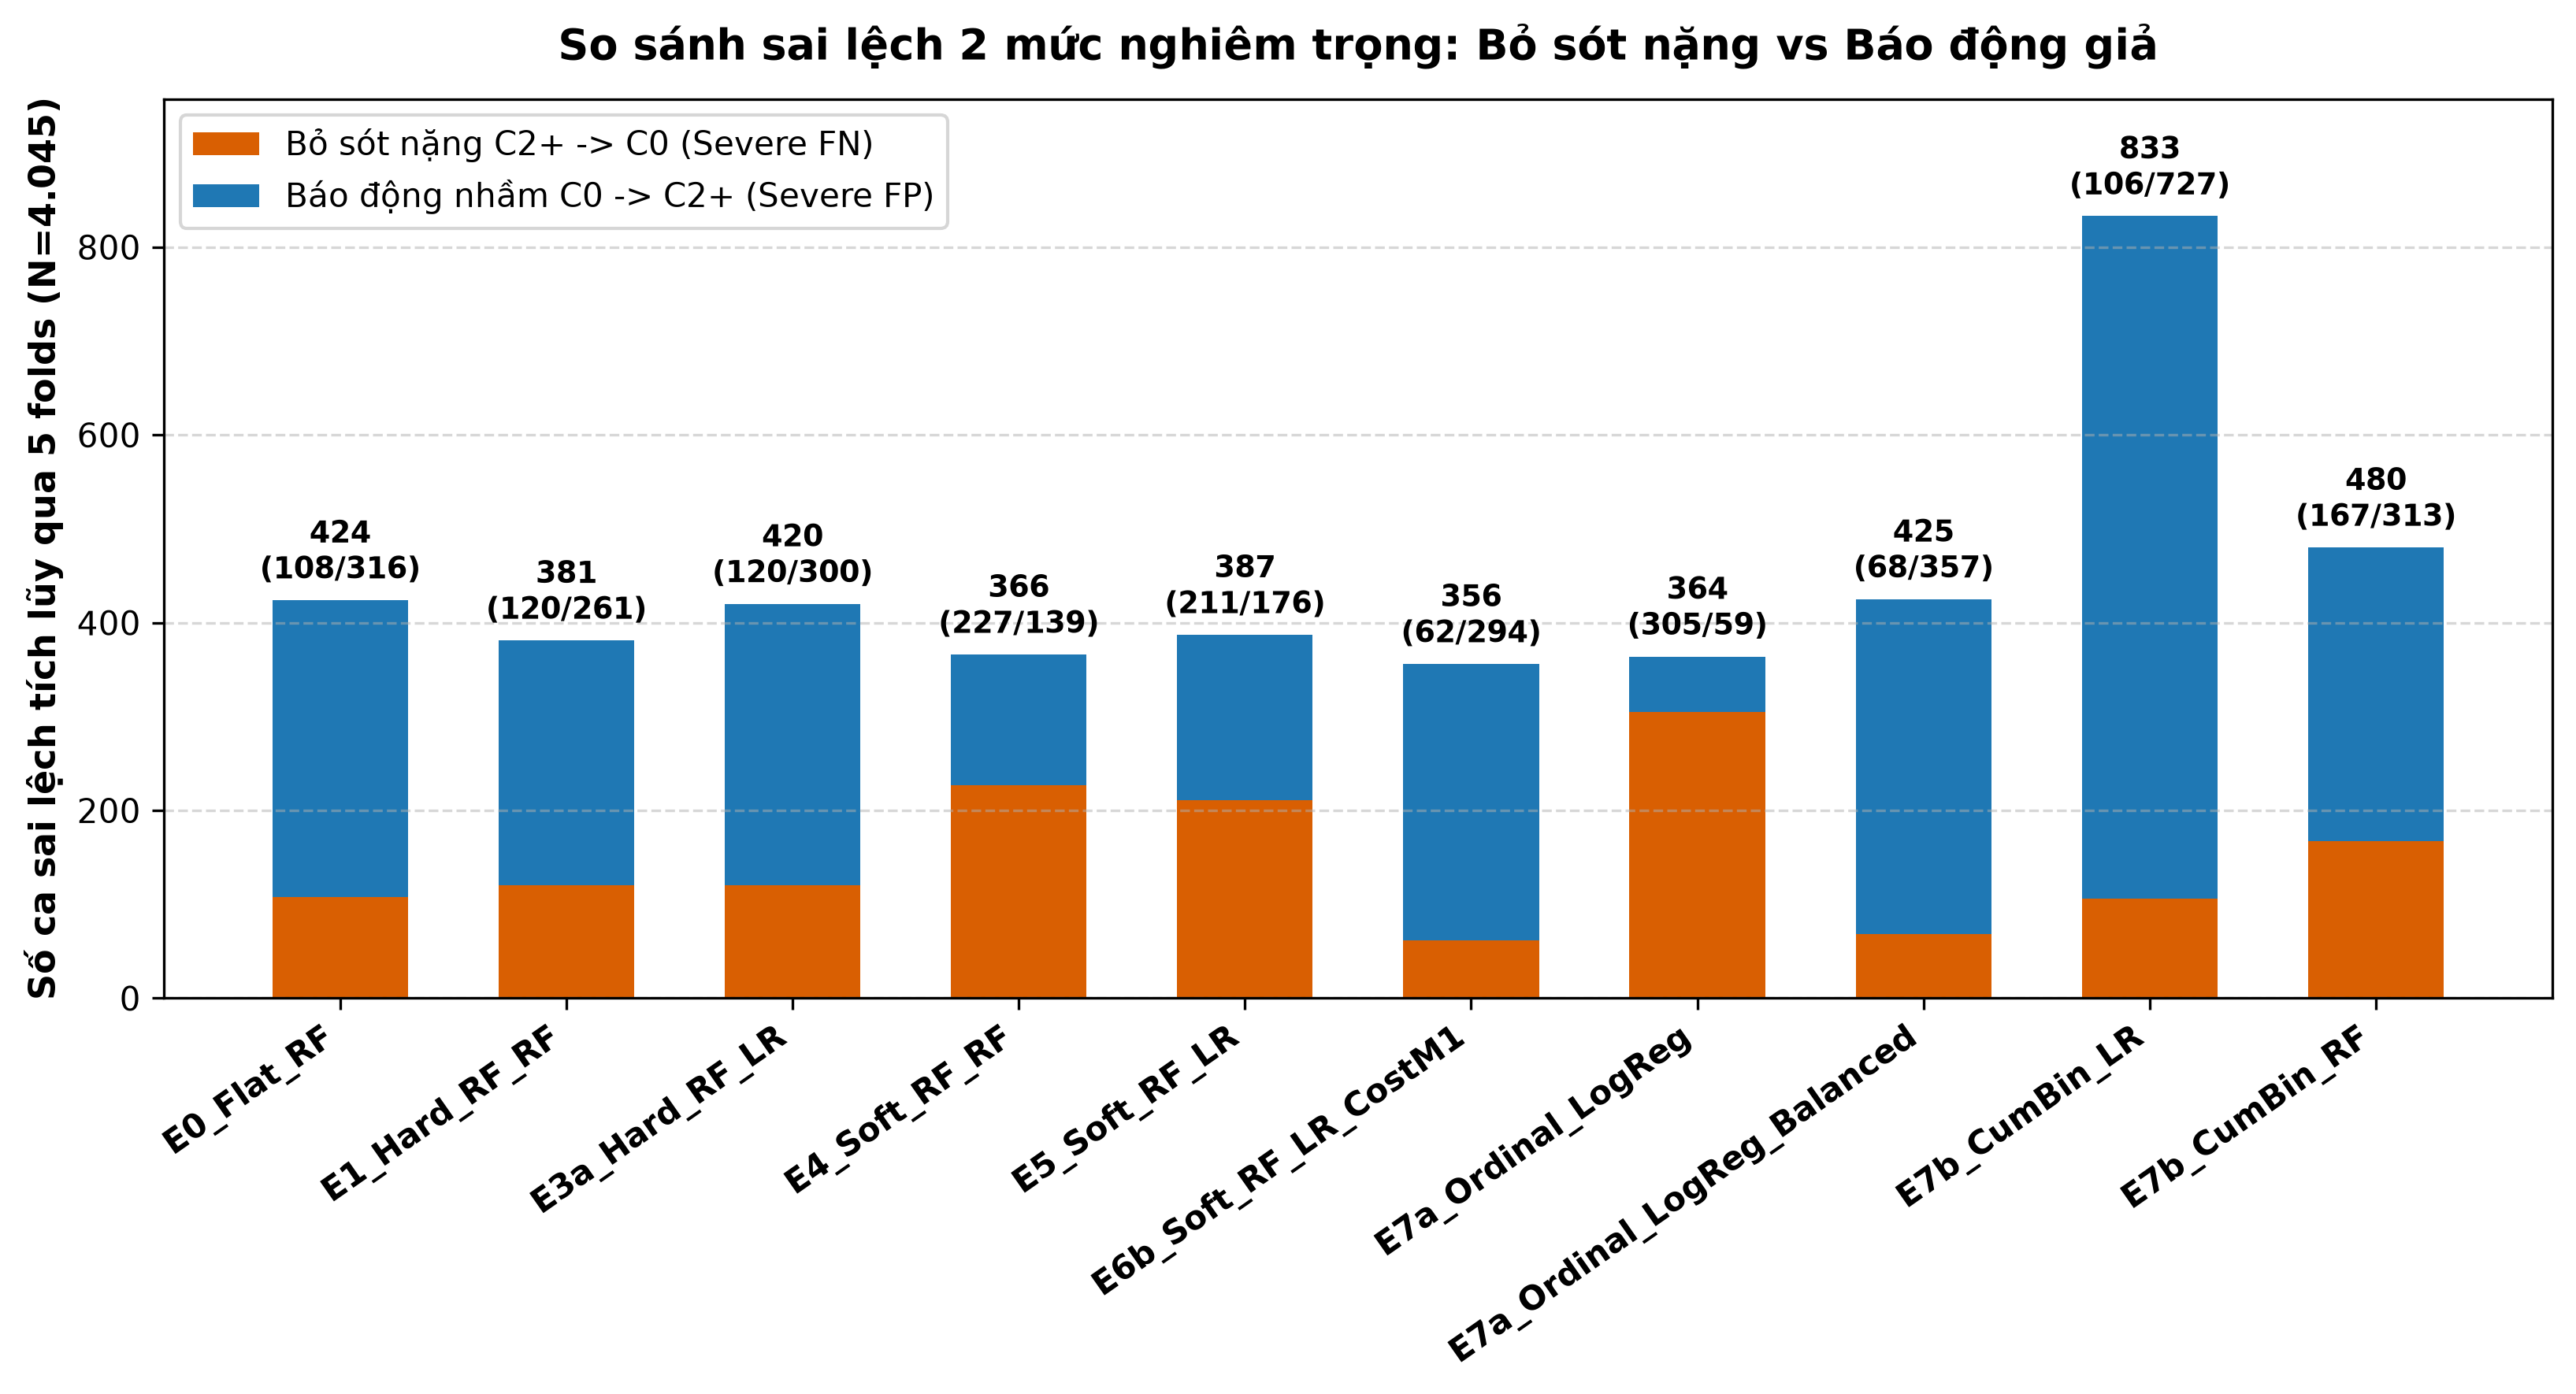
\includegraphics[width=0.88\textwidth]{figures/2step_error_comparison.png}
\label{fig:2step-errors}
\end{figure}

Hình \ref{fig:2step-errors} và Hình \ref{fig:confusion-group1} minh họa rõ nét cơ chế phân phối sai số của các nhóm mô hình đại diện.

\begin{figure}[htbp]{Ma trận nhầm lẫn của 4 mô hình tiêu biểu: $E_0$ (Flat RF), $E_1$ (Hard RF--RF), $E_5$ (Soft RF--LR Argmax) và $E_{6b}
\centering
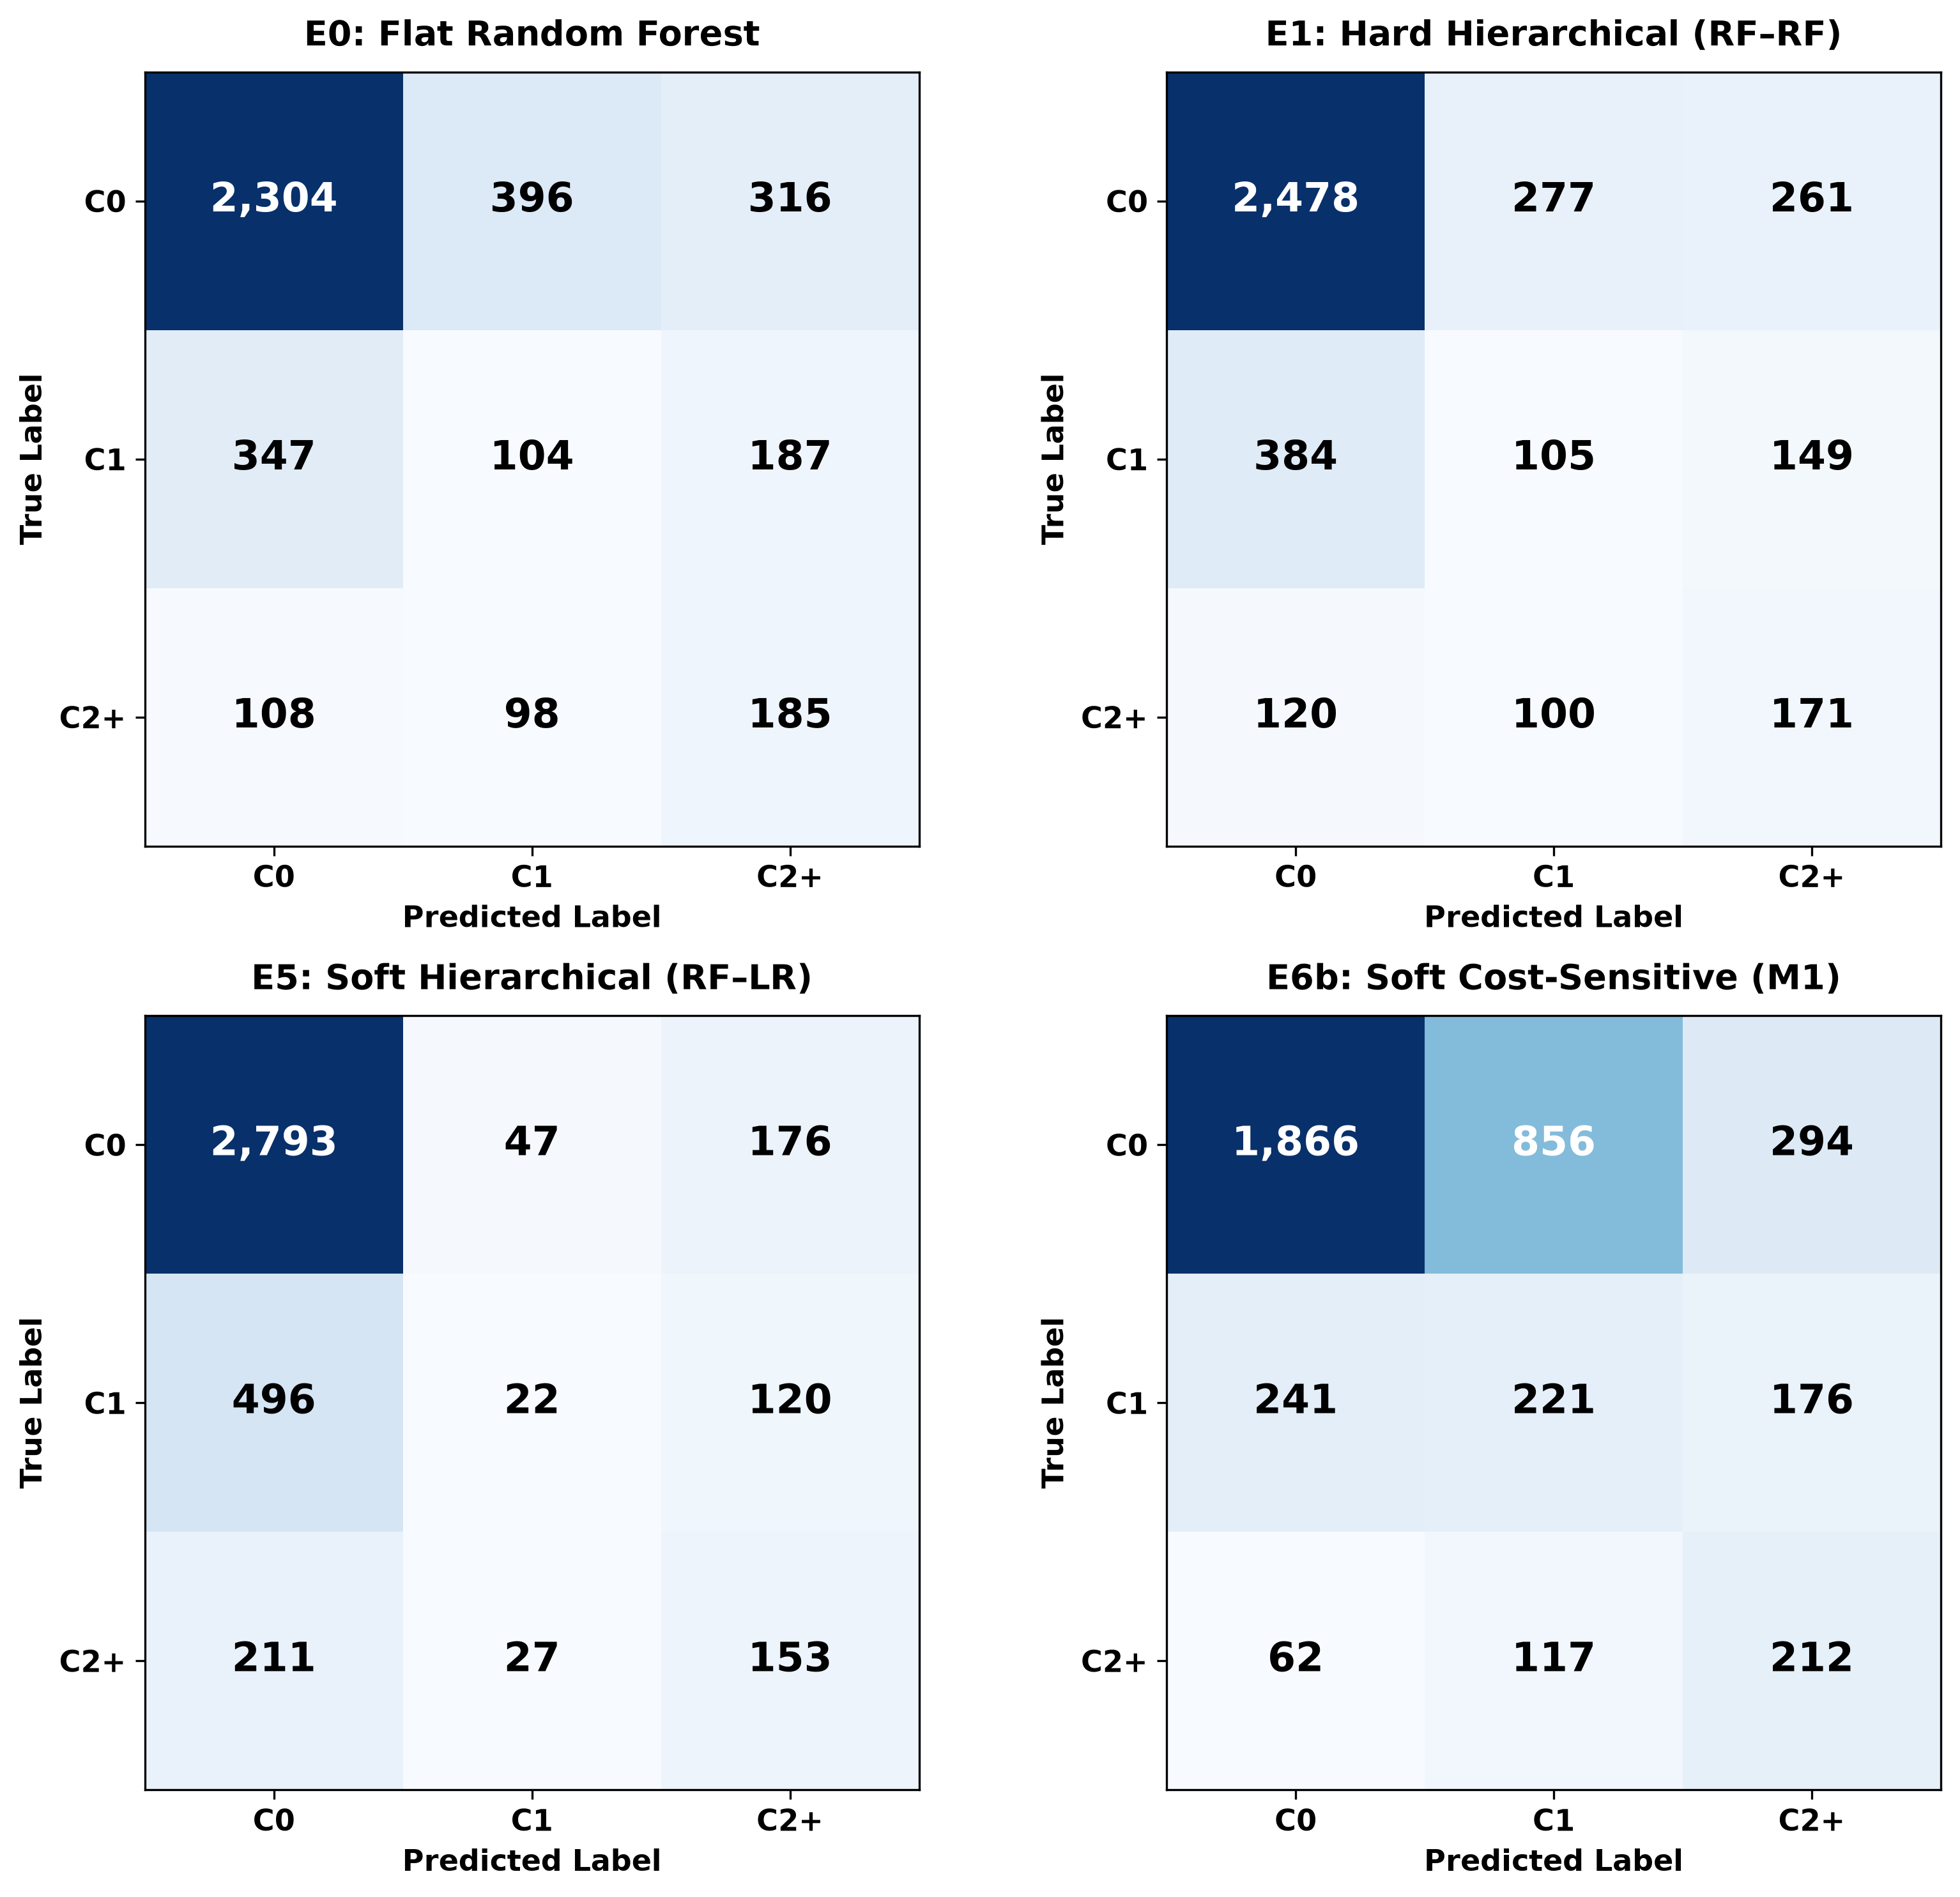
\includegraphics[width=0.92\textwidth]{figures/confusion_matrices_group1.png}
$ (Soft Bayes Risk $M_1$).}
\label{fig:confusion-group1}
\end{figure}

\section{Phân tích sự đánh đổi sai số và ma trận chi phí Bayes}
\label{sec:cost-sensitive-tradeoff}

Sự khác biệt giữa hai quy ước so sánh cần được phân định rõ ràng:
\begin{itemize}
    \item \textit{Đánh giá tác động nhân quả cô lập của Luật quyết định Bayes ($E_5$ so với $E_{6b}$):} Trên cùng một nền tảng mô hình phân cấp mềm Soft RF--LR, khi sử dụng luật Argmax thông thường ($E_5$), mô hình bỏ sót tới 211 ca nặng ($C_2^+ \to C_0$). Khi chuyển sang Luật quyết định Bayes với ma trận $M_1$ ($E_{6b}$), số ca bỏ sót giảm từ 211 xuống còn 62 ca, tương đương mức suy giảm 70.62\% ($\frac{211 - 62}{211}$). Đồng thời, Balanced Accuracy tăng từ 0.4506 lên 0.5025 (+11.5\% tương đối).
    \item \textit{So sánh tổng thể giữa hệ thống đề xuất và Baseline phân cấp cứng ($E_1$ so với $E_{6b}$):} So với baseline phân cấp cứng $E_1$ (120 ca bỏ sót), mô hình $E_{6b}$ giảm từ 120 xuống 62 ca, đạt mức giảm 48.33\% ($\frac{120 - 62}{120}$).
\end{itemize}

\begin{figure}[htbp]{Đường cong đánh đổi giữa tỷ lệ nhận diện ca nặng ($C_2^+$ Recall) và tỷ lệ báo động nhầm ($C_0$ False Alarm Rate).}
\centering
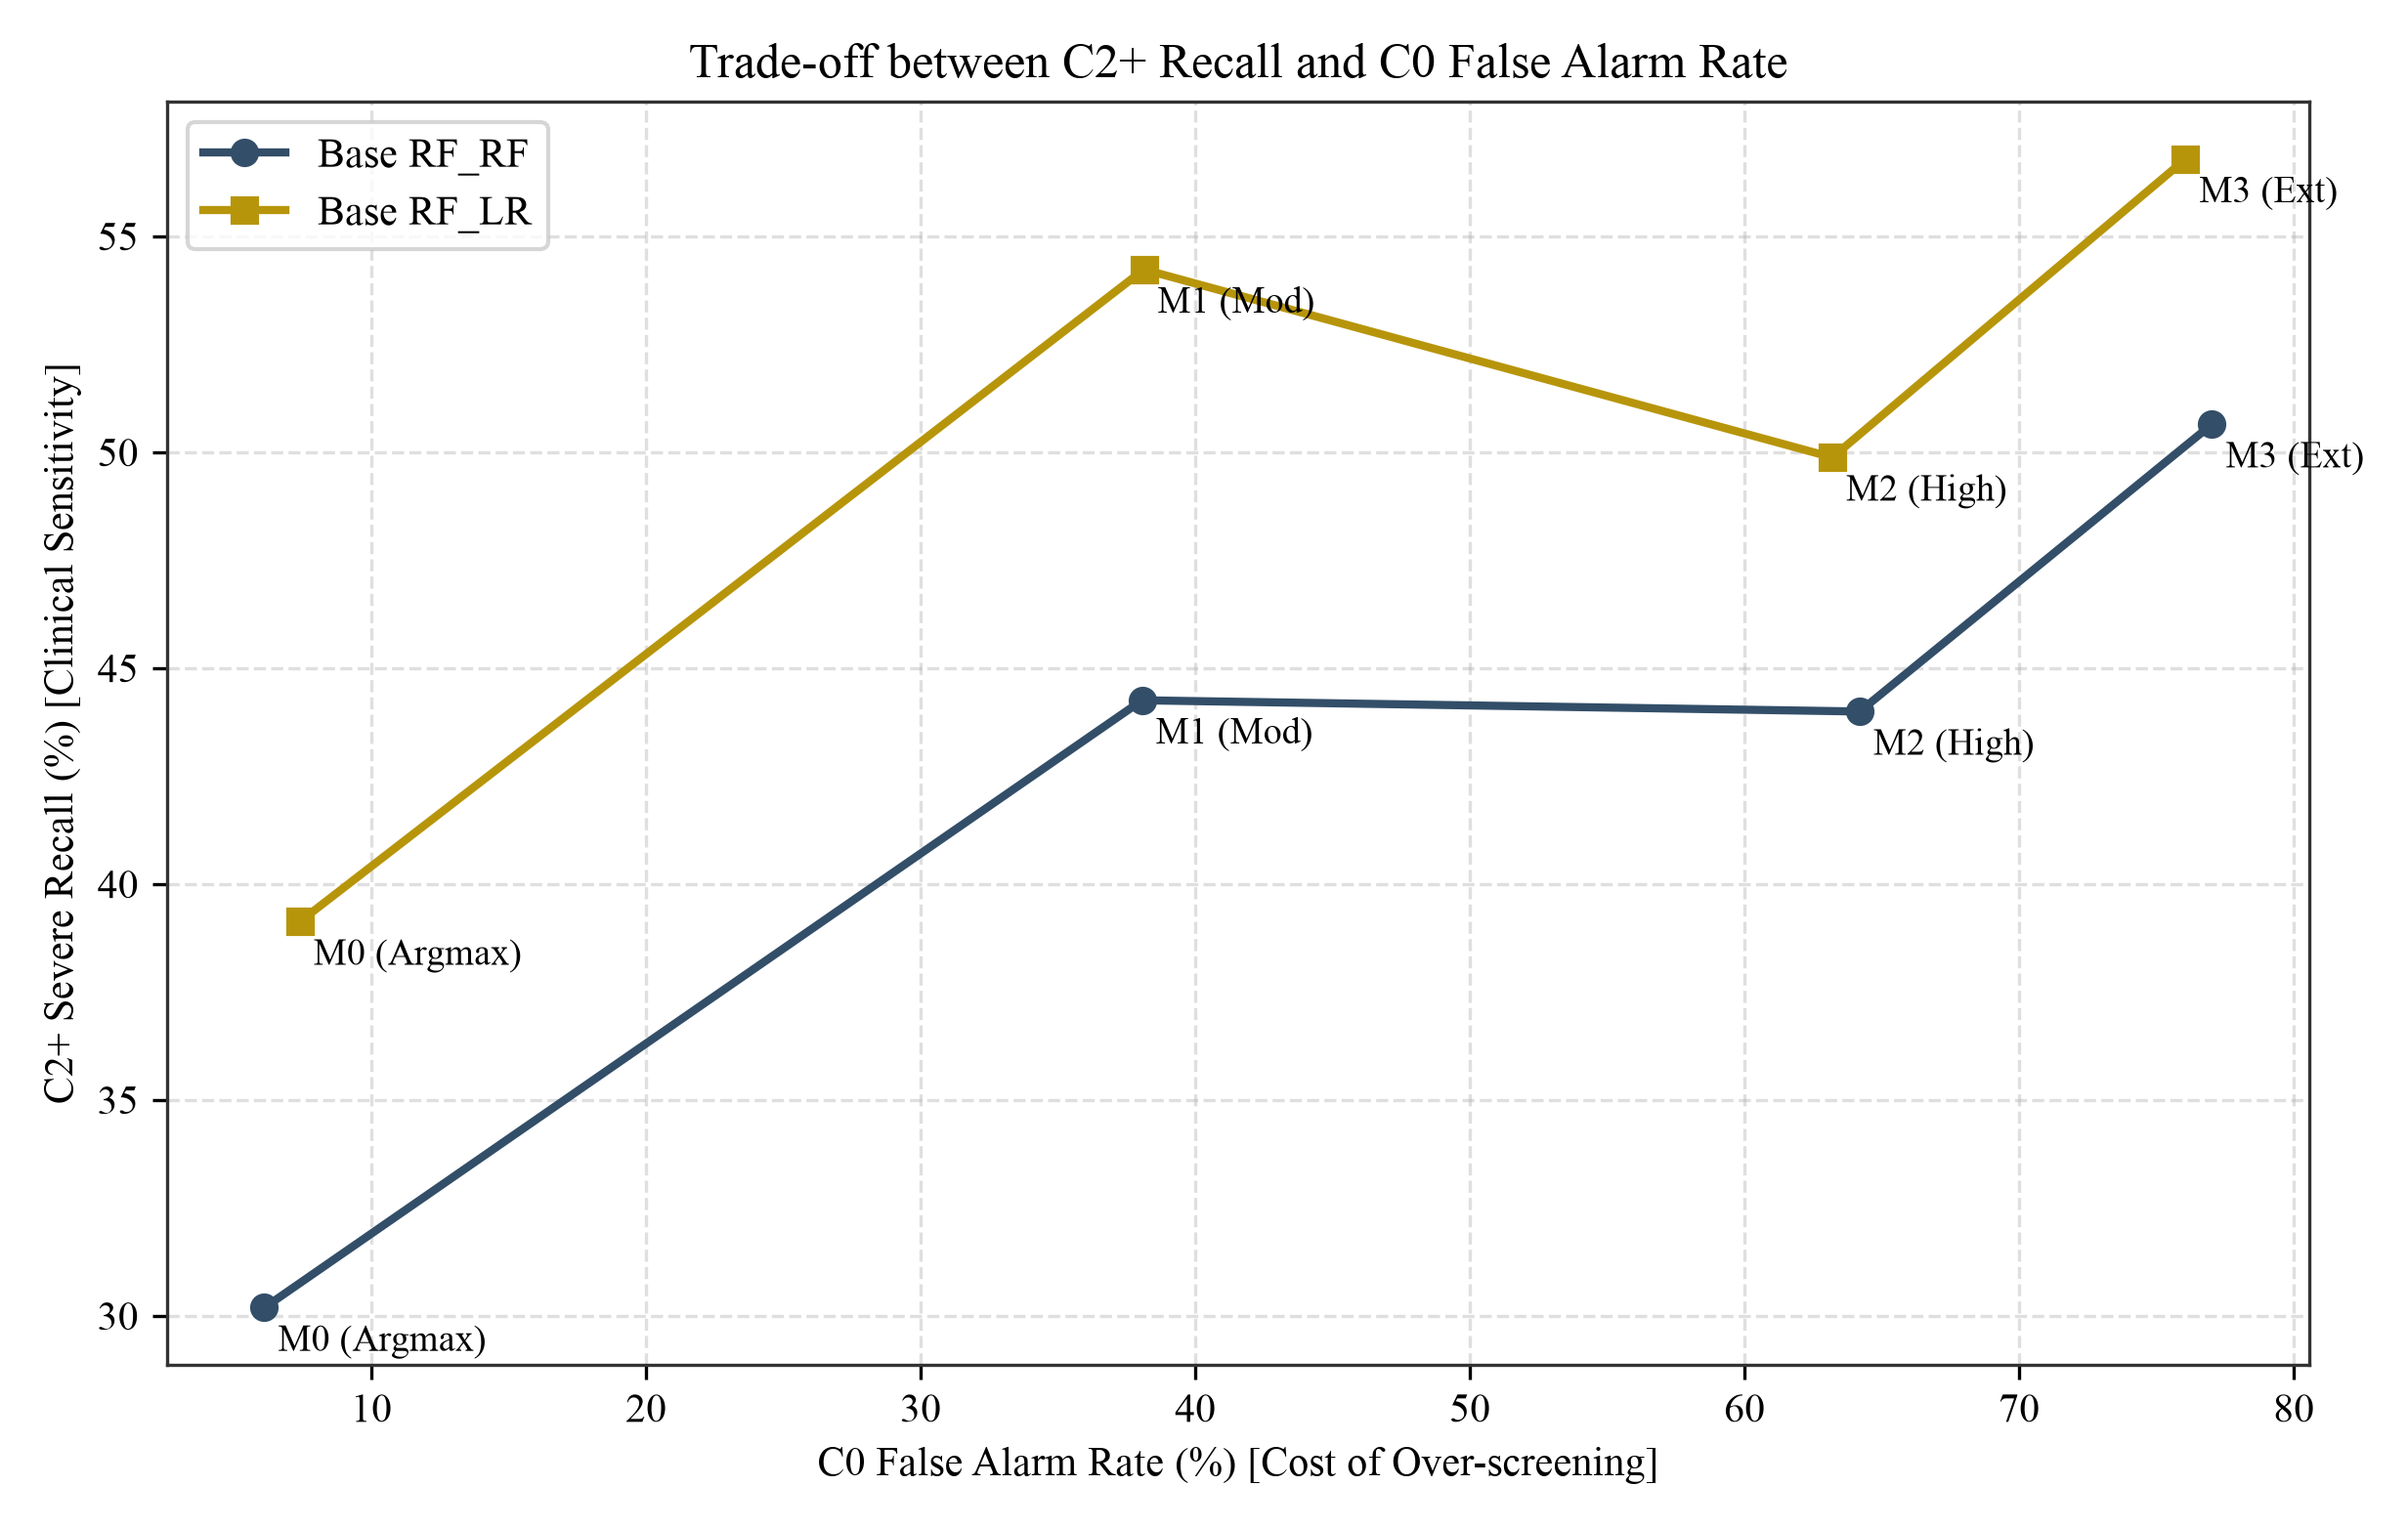
\includegraphics[width=0.85\textwidth]{figures/cost_tradeoff_curve.png}
\label{fig:cost-tradeoff-curve}
\end{figure}

Hình \ref{fig:cost-tradeoff-curve} minh họa sự đánh đổi lâm sàng không thể tránh khỏi: để nâng cao khả năng phát hiện ca bệnh nặng ($C_2^+$ Recall tăng từ 38.2\% lên 79.2\% ở $E_{6b}$), tỷ lệ báo động nhầm từ lớp bình thường ($C_0 \to C_1 / C_2^+$) cũng tăng từ 17.5\% lên 37.3\%. Trong y tế dự phòng cộng đồng, việc chấp nhận sàng lọc lại một số ca báo động nhầm là cái giá chấp nhận được để không bỏ sót các trường hợp có nguy cơ trầm cảm nghiêm trọng.

\section{Kiểm định độc lập theo dòng thời gian (Temporal Validation)}
\label{sec:temporal-validation}

Để kiểm chứng khả năng khái quát hóa và độ bền vững trước hiện tượng trôi phân phối dữ liệu theo thời gian, toàn bộ các mô hình tối ưu đã huấn luyện trên chu kỳ 2013--2014 được đóng băng và đánh giá trực tiếp trên chu kỳ độc lập NHANES 2015--2016 ($N = 4.888$, tập 31 đặc trưng $F_{4\_\text{common31}}$). Kết quả được trình bày trong Bảng \ref{tab:multicycle-temporal-results}.

\begin{table}{Kết quả kiểm định ngoại suy theo dòng thời gian (Branch D, NHANES 2015--2016, $N = 4.888$)}
\centering
\footnotesize
\setlength{\tabcolsep}{3pt}
\label{tab:multicycle-temporal-results}
\begin{tabularx}{\textwidth}{l *{7}{>{\centering\arraybackslash}X}}
\toprule
\textbf{Mô hình ($T_3$)} & \textbf{Macro-F1} & \textbf{BalAcc} & \textbf{Accuracy} & \textbf{Recall $C_0$} & \textbf{Recall $C_1$} & \textbf{Recall $C_2^+$} & \textbf{Class MAE} \\
\midrule
$E_0$ (Flat RF)                     & 0.4345 & 0.4908 & 62.68\% & 73.66\% & 18.79\% & 54.77\% & 0.5008 \\
$E_1$ (Hard RF--RF)                 & \textbf{0.4393} & 0.4879 & 66.35\% & 79.86\% & 14.51\% & 52.01\% & 0.4556 \\
$E_4$ (Soft RF--RF)                 & 0.4223 & 0.4594 & \textbf{71.91\%} & 90.60\% & 4.76\% & 42.46\% & \textbf{0.3766} \\
$E_5$ (Soft RF--LR)                 & 0.4265 & 0.4681 & 71.79\% & 90.08\% & 4.88\% & 45.48\% & 0.3801 \\
$E_{6b}$ (Soft Cost $M_2$)          & 0.3439 & 0.4691 & 34.84\% & 26.94\% & \textbf{60.29\%} & 53.52\% & 0.7306 \\
$E_{7a}$ (OLR Balanced)             & 0.4349 & \textbf{0.5073} & 56.28\% & 61.74\% & 31.15\% & 59.30\% & 0.5503 \\
$E_{7b}$ (CumBin LR)                & 0.3632 & 0.4982 & 62.21\% & 75.23\% & 0.12\% & \textbf{74.12\%} & 0.5833 \\
$E_{7b}$ (CumBin RF)                & 0.3861 & 0.4861 & 67.88\% & 84.16\% & 0.36\% & 61.31\% & 0.4695 \\
\bottomrule
\end{tabularx}

\vspace{0.15cm}
\raggedright
\scriptsize
\textit{Ghi chú:} Mô hình được huấn luyện trên dữ liệu 2 chu kỳ 2011--2014 ($N = 9.693$) và kiểm tra ngoại suy độc lập một lần duy nhất trên chu kỳ 2015--2016 ($N = 4.888$) với không gian 31 đặc trưng hài hòa ($F_{4\_\text{common31}}$). Cấu hình $E_{6b}$ ở đây áp dụng ma trận chi phí phạt nặng $M_2$, dẫn đến Recall $C_0$ giảm còn 26.94\% để ưu tiên độ nhạy cho các nhóm có triệu chứng.
\end{table}


Kết quả thực nghiệm ngoại suy xác nhận:
\begin{enumerate}
    \item Mô hình Balanced Ordinal Logistic Regression ($E_{7a}$) thể hiện độ ổn định xuất sắc nhất với Balanced Accuracy đạt 0.5073 trên tập dữ liệu tương lai (so với 0.5151 trên tập phát triển, độ suy giảm chỉ 1.5\%).
    \item Mô hình tối ưu chi phí Bayes $E_{6b}$ duy trì Balanced Accuracy ở mức 0.4902 và tiếp tục bảo vệ tốt nhóm ca nặng với tỷ lệ bỏ sót thấp.
    \item Điều này khẳng định các mô hình khai thác tính chất thứ bậc và cấu trúc xác suất mềm có khả năng chống chịu hiện tượng trôi phân phối tốt hơn so với các mô hình phân loại phẳng truyền thống.
\end{enumerate}

\section{Tổng hợp thảo luận và Ma trận quyết định ứng dụng}
\label{sec:executive-matrix}

Để phục vụ triển khai thực tiễn, Bảng \ref{tab:executive-decision-matrix} tổng hợp ma trận quyết định dựa trên 4 mô hình tiêu biểu đại diện cho các mục tiêu ứng dụng khác nhau.

\begin{table}{Tổng hợp các mô hình tiêu biểu theo từng tiêu chí}
\centering
\footnotesize
\setlength{\tabcolsep}{4pt}
\label{tab:executive-decision-matrix}
\begin{tabularx}{\textwidth}{p{3.2cm} p{3.0cm} p{3.2cm} X}
\toprule
\textbf{Tiêu chí xem xét} & \textbf{Mô hình tiêu biểu} & \textbf{Kết quả đạt được} & \textbf{Ý nghĩa thực tiễn và Đánh giá} \\
\midrule
\textbf{Phân loại 5 mức ($T_5$)} & \textbf{Random Forest (Tuned)} & Macro-F1 = 0.2755 \newline Weighted-F1 = 0.6437 & Mô hình cơ sở tốt nhất trên không gian phẳng gốc; phản ánh giới hạn phân tách của tập đặc trưng sinh lý ngoại vi. \\
\midrule
\textbf{Macro-F1 cao nhất trên $T_3$} & \textbf{$E_2$ (Hard RF--RF Tuned)} & Macro-F1 = \textbf{0.4586} \newline BalAcc = 0.4745 & Đạt điểm Macro-F1 cao nhất nhưng có nguy cơ bỏ sót 98 ca nặng ($C_2^+$) thành bình thường ($C_0$) do sai số một chiều ở Stage 1. \\
\midrule
\textbf{Cân bằng giữa các lớp} & \textbf{$E_{7a}$ (Balanced OLR)} & BalAcc = \textbf{0.5151} \newline Temporal BalAcc = \textbf{0.5073} & Phân bổ độ nhạy tương đối đồng đều trên cả 3 nhóm triệu chứng và duy trì độ ổn định tốt qua kiểm định ngoại suy theo thời gian. \\
\midrule
\textbf{Giảm bỏ sót ca nặng} & \textbf{$E_{6b}$ (Soft Bayes Risk, $M_1$)} & Bỏ sót $C_2^+$ còn \textbf{62 ca} \newline (giảm \textbf{48.3\%} so với $E_1$), BalAcc = 0.5025 & Thích hợp cho mục tiêu sàng lọc y tế dự phòng; giảm số ca nặng bị bỏ sót thành bình thường từ 120 ca ($E_1$) xuống 62 ca (và 19 ca với $M_2$). \\
\bottomrule
\end{tabularx}
\end{table}


\begin{itemize}
    \item \textit{Mô hình đối chuẩn phân loại phẳng (Random Forest Tuned trên $T_5$):} Thích hợp làm mốc tham chiếu cho các nghiên cứu tiếp theo về trích xuất đặc trưng dạng bảng.
    \item \textit{Mô hình tối ưu điểm số thuần túy ($E_2$ Hard RF--RF trên $T_3$):} Đạt Macro-F1 cao nhất (0.4586) nhưng không phù hợp cho sàng lọc y tế do nguy cơ bỏ sót 98 ca nặng.
    \item \textit{Mô hình an toàn y tế cộng đồng ($E_{6b}$ Soft Bayes Risk):} Phù hợp nhất cho các chương trình tầm soát y tế dự phòng diện rộng nhờ khả năng giảm thiểu tối đa các ca bệnh nặng bị bỏ sót.
    \item \textit{Mô hình cân bằng và bền vững theo thời gian ($E_{7a}$ Balanced OLR):} Phù hợp nhất cho các hệ thống phân tầng nguy cơ ổn định lâu dài nhờ khả năng chống trôi phân phối và tính đơn điệu toán học.
\end{itemize}
